\documentclass[../main.tex]{subfiles}






\begin{document}

\chapter{El grup fonamental}











\section{El grup fonamental}
\begin{defi}
[Camí tancat o llaç]\index{Camí tancat}\index{Llaç}\label{def:camitancat}\label{def:llaç} Un camí que comença i acaba en un mateix punt s'anomena \textit{camí tancat} o \textit{llaç}. 
\end{defi}

\begin{defi}
[Grup fonamental]\label{def:grupfonamental}\index{Grup fonamental} El grup fonamental d'un espai topològic $X$ amb punt base $p$ és el conjunt $\pi(X,p)$ de classes d'homotopia (relativa als extrems) de llaços $\sigma:I\rightarrow X$, amb $\sigma(0) = \sigma(1)=p$.
\end{defi}

\begin{prop}[Exercici 1]
\label{prop:grupfonamental}\label{exercici2.1} El grup fonamental\footnote{També se li diu \textit{grup de Poincaré}\index{Grup de Poincaré} o \textit{primer grup d'homotopia}\index{Primer grup d'homotopia}.} $\pi(X,p)$ és, en efecte, un grup.
\end{prop}
\begin{proof}
\begin{enumerate}[(i)]
    \item \underline{Producte ben definit}. Demostrem que si $\sigma,\sigma',\omega$ i $\omega'$ són camins en un espai $X$ tals que $\sigma(0)=\sigma'(0)$, $\sigma(1) = \sigma'(1)=\omega(0)=\omega'(0)$, $\omega(1) = \omega'(1)$ amb $\sigma\simeq \sigma'$ i $\omega\simeq \omega'$, llavors es compleix que $\sigma*\omega\simeq \sigma'*\omega'$. D'aquesta manera, el producte de classes definit anteriorment està ben definit perquè no dependrà del representant de classe.
    \begin{equation}
        \notag
        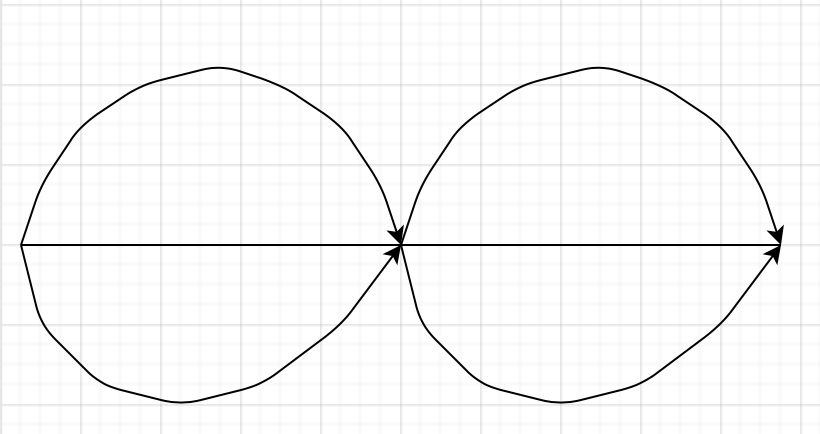
\includegraphics[scale=0.3]{fotos_topo_2/otrasfotos/quatrecamins.png}
    \end{equation}
    Anomenem $F:\sigma\simeq \sigma'$ i $G:\omega\simeq\omega'$ i donem l'homotopia $H:[0,1]\times[0,1]\rightarrow X$, $H_t = F_t*G_t$, és a dir,
    \begin{equation}
        \notag
        H(s,t) = \left\{
        \begin{array}{rcl}
            F(2s,t) & \mathrm{si} & 0\leq s\leq \frac{1}{2}\\
            G(2s-1,t) & \mathrm{si} & \frac{1}{2}\leq s\leq 1
        \end{array}
        \right.
    \end{equation}
    Per $t=0$, tenim:
    \begin{equation}
        \notag
        H(s,0) = \left\{
        \begin{array}{rcl}
            H(s,0) = F(2s,0) = \sigma(2s) & \mathrm{si} & 0\leq s\leq 1/2 \\
            H(s,1) = G(2s-1,0)=\omega(2s-1) & \mathrm{si} & 1/2\leq s\leq 1
        \end{array}
        \right.
    \end{equation}
    Per tant, $H(s,0) = (\sigma*\omega)(s)$. Anàlogament $H(s,1)=(\sigma'*\omega')(s)$. A més,
    \begin{equation}
        \notag
        \begin{array}{ll}
            F(1,t) = q\quad \forall t\\
            G(0,t) = q\quad \forall t
        \end{array}
    \end{equation}
    Finalment, cal veure que els extrems són fixos, és a dir, que és una homotopia relativa als extrems.
    \begin{equation}
        \notag
        \begin{array}{ll}
            H(0,t)=F(0,t)=F_t(0) = p & \forall t \\
            H(1,t) = G(1,t)=G_t(1) = r & \forall t
        \end{array}
    \end{equation}
    Per tant, tenim l'homotopia entre $\sigma*\omega$ i $\sigma'*\omega'$.
    
    \item \underline{Producte associatiu}. Demostrem que si $\sigma,\omega,\tau$ són camins en $X$ tal que $\sigma(1) = \omega(0)$ i $\omega(1) = \tau(0)$, llavors $(\sigma*\omega)*\tau\simeq \sigma*(\omega*\tau)$.
    \begin{equation}
        \notag
        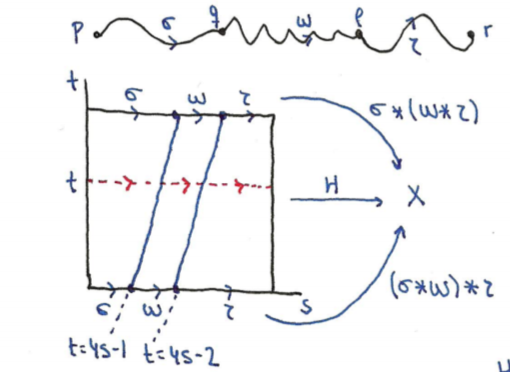
\includegraphics[scale = 0.9]{fotos_topo_2/otrasfotos/manypaths.png}
    \end{equation}
    Prenem $H:[0,1]\times[0,1]\rightarrow X$ definida com
    \begin{equation}
        \notag
        H(s,t) = \left\{
        \begin{array}{rl}
            \sigma\left(\dfrac{4s}{1+t}\right)& 0\leq s\leq \frac{1}{4}(1+t) \\
            \omega(4s-1-t) & \frac{1}{4}(1+t)\leq s\leq \frac{1}{4}(2+t) \\
            \tau\left(\dfrac{4s-2-t}{2-t}\right) & \frac{1}{4}(2+t)\leq s\leq 1
        \end{array}
        \right.
    \end{equation}
    Ràpidament es verifica que $H$ és contínua, que $H(0,t) = \sigma(0)=p$, $H(1,t) = \tau(1)=r$ i que
    \begin{equation}
        \notag
        H\left(\frac{t+1}{4},t\right) = \sigma\left(\frac{t+1}{t+1}\right) = \sigma(1) = q= \omega(0) = H\left(\frac{t+2}{4},t\right).
    \end{equation}
    Finalment, ens queda veure que
    \begin{equation}
        \notag
        H(s,0) = \left\{
        \begin{array}{rl}
            \sigma(4s), & 0\leq s\leq 1/4 \\
            \omega(4s-1), & 1/4\leq s \leq 1/2 \\
            \tau(2s-1),& 1/2\leq s\leq 1
        \end{array}
        \right\} = ((\sigma*\omega)*\tau)(s)
    \end{equation}
    i de manera similar $H(s,1) = (\sigma*(\omega*\tau))(s)$ com volíem. Així doncs, hem demostrat que $\sigma*(\omega*\tau) \simeq (\sigma*\omega)*\tau$ que això vol dir que amb les classes $[\sigma]([\omega][\tau]) = ([\sigma][\omega])[\tau]$, és a dir, que el producte és associatiu. Ara bé, la demostració l'hem fet més general, ja que hem agafat qualssevol camins i no necessàriament llaços. Però serveix igual.
    
    \item \underline{Element neutre}. Denotem per $c_p$ el camí a $X$ constant en el punt $p$, és a dir, que $\forall t\in [0,1]$, $c_p(t) = p$. Aquest serà el nostre element neutre. Anem a veure-ho. En efecte, si $\sigma$ és un camí qualsevol, aleshores $c_{\sigma(0)}*\sigma\simeq \sigma$ i $\sigma*c_{\sigma(1)}\simeq \sigma$. Aleshores, passant a la classe, el camí constant no dependrà del punt. Veiem aquestes homotopies si es compleixen. Definim
    \begin{equation}
        \notag
        H(s,t) = \left\{
        \begin{array}{rcl}
            p & \mathrm{si} & 0\leq s\leq \frac{1}{2}(1-t) \\
            \sigma\left(\dfrac{2s-1-t}{1+t}\right) & \mathrm{si} & \frac{1}{2}(1-t)\leq s\leq 1
        \end{array}
        \right.
    \end{equation}
    i amb això aconseguim la primera homotopia de camins. Anàlogament, 
    \begin{equation}
        \notag
        H(s,t) = \left\{
        \begin{array}{rcl}
            \sigma\left(\dfrac{2s}{1+t}\right) & \mathrm{si} & 0\leq s\leq \frac{1}{2}(1+t) \\
            q & \mathrm{si} & \frac{1}{2}(1+t)\leq s\leq 1
        \end{array}
        \right.
    \end{equation}
    ens dona la segona.
    \item \underline{Element invers}. Donat un element $[\sigma]$ el seu invers és la classe del camí definit per $\overline{\sigma}(t) = \sigma(1-t)$. En efecte, si definim
    \begin{equation}
        \notag
        H(s,t) = \left\{
        \begin{array}{rcl}
            \sigma(2s) & \mathrm{si} & 0\leq s\leq \frac{1-t}{2} \\
            \sigma(1-s) & \mathrm{si} & \frac{1-t}{2}\leq s\leq \frac{1+t}{2} \\
            \sigma(2-2s) & \mathrm{si} & \frac{1+t}{2}\leq s\leq 1
        \end{array}
        \right.
    \end{equation}
    obtenim que $\sigma*\overline{\sigma}\simeq c_{\sigma(0)}$, que implica que $[\sigma][\overline{\sigma}]=[c_p]$. D'altra banda, com que $\overline{\overline{\sigma}} = \sigma$, obtenim que $\overline{\sigma}*\sigma\simeq c_{\sigma(1)}$ i així provem que $[\overline{\sigma}]$ és l'element invers de $[\sigma]$ a $\pi(X,p)$.
\end{enumerate}
Amb això provem que $\pi(X,p)$ és un grup.
\end{proof}

Així doncs, hem format un grup amb tots els llaços que són essencialment diferents, és a dir, que no es poden transformar els uns en els altres, mitjançant unes transformacions contínues (veure \ref{def:homotopiadecamins}). En definitiva:
\begin{equation}
    \notag
    \pi(X,p) = \{[\sigma]\;:\;\sigma:I\rightarrow X,\;\sigma(0)=\sigma(1)=p\}.
\end{equation}

\begin{ej}
\label{ej:grupfonamentalder} Sigui $X = \mathbb{R}^2$ i $p = (0,0)$, anem a veure què és $\pi(X,p)$. Sigui $\alpha:[0,1]\rightarrow \mathbb{R}^2$ tal que $\alpha(0) = \alpha(1) = p$. Considerem $F:[0,1]\times [0,1]\rightarrow \mathbb{R}^2$ tal que $F(t,s) = \alpha(t)s+(1-s)p$. Aleshores aquesta aplicació és contínua i està ben definida. També podem observar com $F(t,0) = p = \varepsilon_p$ i $F(t,1) = \alpha(t)$ per a tot $5\in[0,1]$ i que $F(0,s) = \alpha(0)s+(1-s)p = ps+p-ps = p$ i $F(1,s) = \alpha(1)s+(1-s)p = p$. Per tant, $F$ defineix una homotopia entre $\alpha$ i $\varepsilon_p$ relativa a $\{0,1\}$ per tant $[\alpha] = [\varepsilon_p]$. Aleshores podem concloure que $\pi(\mathbb{R}^2,(0,0)) = [\varepsilon_p]\cong \{0\}$, el grup trivial.
\end{ej}

\section{Canvi de punt base}

Per la seva pròpia definició, el grup fonamental depèn, en principi, de l'elecció del punt base de l'espai topològic que ens ocupi. Però ara veurem que, de fet, tan sols és sensible a la component arc-connexa de $X$ en què es troba el punt. És a dir, el grup fonamental d'un espai topològic $X$ amb punt base $p$, no dependrà de $p$, sinó que dependrà de la component arc-connexa de $p$.

\begin{ter}
[Canvi de punt base]\label{ter:canvidepuntbase} Si $p$ i $p'$ són dos punts d'un mateix espai topològic $X$ que pertanyen a la mateixa component arc-connexa. Aleshores $\pi(X,p)\cong \pi(X,p')$.
\end{ter}
\begin{proof}
Suposem que aquests dos punts $p$ i $p'$ pertanyen a la mateixa component arc-connexa. Aleshores podem establir un camí $\gamma:I\rightarrow X$ de forma que vagi de $p$ a $p'$, és a dir, que $\gamma(0) = p$ i $\gamma(1) =p'$. Denotem per $\overline{\gamma}$ el camí invers, és a dir, $\overline{\gamma}(t) = \gamma(1-t)$.

Ara definim l'aplicació
\begin{equation}
    \notag
    u_\gamma:\pi(X,p)\rightarrow \pi(X,p'),\quad u_\gamma([\alpha]) = [\overline{\gamma}*\alpha*\gamma].
\end{equation}
Observem que, com que $(\overline{\gamma}*\alpha)*\gamma\simeq\overline{\gamma}*(\alpha*\gamma)$, no cal que especifiquem parèntesis en l'expressió $[\overline{\gamma}*\alpha*\gamma]$.

Doncs bé, si provem que aquesta aplicació és un isomorfisme de grups, obtindrem el que volem. Per veure això, cal veure que $u_\gamma$ està ben definida, que és un morfisme de grups i per últim que és isomorfisme.
\begin{itemize}
    \item \underline{Està ben definida}. Suposem que $[\sigma]=[\sigma']$, és a dir, $\sigma\simeq\sigma'$. Llavors, com que ja sabem que la composició de camins és compatible amb la relació d'homotopia, deduïm que $\overline{\gamma}*\sigma\simeq\overline{\gamma}*\sigma'$ i a continuació $(\overline{\gamma}*\sigma)*\gamma\simeq(\overline{\gamma}*\sigma')*\gamma$. Per tant, $[\overline{\gamma}*\sigma*\gamma]=[\overline{\gamma}*\sigma'*\gamma]$ i per tant està ben definida.
    
    \item \underline{És morfisme de grups}. Cal demostrar que $u_\gamma([\sigma][\omega]) = u_\gamma([\sigma])u_\gamma([\omega])$, on $\sigma,\omega$ són dos llaços en el punt $p$. Observem que d'una banda tenim
    \begin{equation}
        \notag
        u_\gamma([\sigma][\omega]) = u_\gamma([\sigma*\omega])=[\overline{\gamma}*\sigma*\omega*\gamma],
    \end{equation}
    mentre que d'altra banda tenim
    \begin{equation}
        \notag
        u_\gamma([\sigma])u_\gamma([\omega])=[\overline{\gamma}*\sigma*\gamma][\overline{\gamma}*\omega*\gamma] = [\overline{\gamma}*\sigma*\gamma*\overline{\gamma}*\omega*\gamma]
    \end{equation}
    com que $\gamma*\overline{\gamma}\simeq \varepsilon_p$ (on $\varepsilon_p$ denota el camí constant en $p$), deduïm que
    \begin{equation}
        \notag
        [\overline{\gamma}*\sigma\gamma*\overline{\gamma}*\omega*\gamma] = [\overline{\gamma}*\sigma*\omega*\gamma]
    \end{equation}
    i aleshores tenim la igualtat que volíem.
    \item \underline{És isomorfisme}. Per demostrar que $u_\gamma$ és un isomorfisme només ens cal ara provar que és una aplicació bijectiva. 
    
    Considerem l'aplicació
    \begin{equation}
        \notag
        u_{\overline{\gamma}}:\pi(X,p')\rightarrow \pi(X,p)
    \end{equation}
    definida com $u_{\overline{\gamma}}([\sigma])= [\gamma*\sigma*\overline{\gamma}]$. Aquesta aplicació és també un morfisme de grups ben definit (la demostració és anàloga a la que hem fet per a $u_\gamma$ utilitzant que $\overline{\overline{\gamma}} = \gamma$. Llavors
    \begin{equation}
        \notag
        u_{\overline{\gamma}}(u_\gamma([\sigma])) = u_{\overline{\gamma}}([\overline{\gamma}*\sigma*\gamma]) = [\gamma*\overline{\gamma}*\sigma\gamma*\overline{\gamma}] = [\varepsilon_p*\sigma*\varepsilon_p]=[\sigma]
    \end{equation}
    per a tot llaç $\sigma$ en $p$. Per tant, la composició $u_{\overline{\gamma}}\circ u_\gamma$ és la identitat. Anàlogament, la composició $u_\gamma\circ u_{\overline{\gamma}}$ també és la identitat. D'aquests dos fets deduïm que $u_\gamma$ i $u_{\overline{\gamma}}$ són aplicacions bijectives, inverses l'una de l'altra. Això demostra el que volíem.
\end{itemize}
I per tant tenim que $\pi(X,p)\cong\pi(X,p')$ mitjançant l'isomorfisme $u_\gamma$.
\end{proof}

\begin{coro}
\label{coro:canvidepuntbase} Si $X$ és un espai arc-connex aleshores per a tota parella de punts $x,y\in X$ es té que $\pi(X,x)\cong \pi(X,y)$
\end{coro}
\begin{proof}
És una conseqüència directa del teorema (\ref{ter:canvidepuntbase}) del canvi de punt base: si $X$ és arc-connex, només té una component arc-connexa a la qual hi pertanyen tots els punts.
\end{proof}

\section{Relació entre grups fonamentals de diferents espais}

\subsection{El grup fonamental és un invariant topològic}

També podem relacionar els grups fonamentals de diferents espais topològics amb punts base. En realitat, es tracta d'una ``extensió'' de l'apartat anterior, en el qual es demostrava que el grup fonamental no depenia del punt base sinó de la component arc-connexa. En aquest cas el que demostrarem és que si tenim dos espais topològics amb punts base i una aplicació entre ells que envia un punt base a l'altre, aleshores els seus grups fonamentals seran isomorfs, sempre i quan els espais topològics siguin homeomorfs.

\begin{prop}
\label{prop:morfismegrupfonamental} Si tenim $X$ i $Y$ espais topològics amb punts fixos $p_x\in X$ i $p_y\in Y$ i tenim l'aplicació contínua $\varphi:X\rightarrow Y$ que satisfà $p_y = \varphi(p_x)$, aleshores
\begin{enumerate}[(1)]
    \item Si $\alpha$ és un camí en $X$, llavors $\varphi\circ\alpha$ és un camí en $Y$.
    \item Si $F$ és una homotopia entre dos camins $\alpha$ i $\beta$ de $X$, llavors $\varphi\circ F$ és una homotopia entre els camins $\varphi\circ\alpha$ i $\varphi\circ\beta$ en $Y$.
    \item L'aplicació $\varphi_*:\pi(X,p_x)\rightarrow \pi(Y,p_y)$ definida per $\varphi_*([\sigma]):=[\varphi\circ\sigma]$ és un morfisme de grups. Se li'n diu \textit{morfisme induït}
\end{enumerate}
\end{prop}
\begin{proof}
Els dos primers punts són trivials. Cal mirar les definicions anteriors d'homotopia de camins. El punt (3) es prova mitjançant els dos primers punts, que ens donen que és una aplicació ben definida. D'altra banda, per veure que és un morfisme prenem dues classes $[\alpha],[\beta]\in\pi(X,p_x)$ qualsevulles i aleshores
\begin{equation}
    \notag
    \varphi_*([\alpha][\beta]) = \varphi_*([\alpha*\beta]) = [\varphi\circ(\alpha*\beta)] = [(\varphi\circ\alpha)\circ(\varphi\circ\beta] =
\end{equation}
\begin{equation}
    \notag
    =[\varphi\circ\alpha][\varphi\circ\beta] = \varphi_*([\alpha])\varphi_*([\beta])
\end{equation}
i per tant és un morfisme de grups.
\end{proof}

Notem, però, que $\varphi_*$ sota aquestes hipòtesis no defineix necessàriament un isomorfisme de grups. Sigui com sigui, la propietat següent dels morfismes induïts serà una pista per veure quines hipòtesis s'hauran d'afegir per a que $\varphi:X\rightarrow Y$ sigui un isomorfisme.

\begin{prop}
\label{prop:transitivitatmorfismeinduit} Donades $\varphi:X\rightarrow Y$ i $\psi:Y\rightarrow Z$ aplicacions contínues entre espais topològics, es compleix que $(\psi\circ\varphi)_* = \psi_*\circ\varphi_*$
\end{prop}
\begin{proof}
Clarament l'aplicació $\psi\circ\varphi:X\rightarrow Z$ és contínua, per ser composició d'aplicacions contínues entre espais topològics. De manera que el morfisme induït és $(\psi\circ\varphi)_*([\alpha])=[(\psi\circ\varphi)\circ\alpha]$, per a qualsevol $\alpha\in\pi(X,p_x)$, on $p_x$ és el punt base de $X$. Aleshores:
\begin{equation}
    \notag
    (\psi\circ\varphi)_*([\alpha]) = [\psi\circ\varphi\alpha] = \psi_*([\varphi\circ\alpha]) = \psi_*(\varphi_*([\alpha]))
\end{equation}
per la propietat de l'associativitat de la composició de funcions. Això prova, doncs, que $(\psi\circ\varphi)_*=\psi_*\circ\varphi_*$ com volíem.
\end{proof}

Ara sí, ja podem demostrar l'isomorfia que busquem.

\begin{ter}
[Invariant topològic]\label{ter:invarianciatopologicadelgrupfonamental} Si $X$, $Y$ són arc-connexos i $X\simeq Y$ (és a dir, són homeomorfs), llavors $\forall x\in X$, $\forall y\in Y$, els grups fonamentals de $(X,x)$ i $(Y,y)$ són isomorfs, és a dir, $\pi(X,x)\cong \pi(Y,y)$.
\end{ter}
\begin{proof}
Fixant els punts base $x\in X$ i $y\in Y$, suposant, sense pèrdua de generalitat que $\varphi:X\rightarrow Y$ és un homeomorfisme que satisfà que $\varphi(x) = y$, existeix una aplicació contínua $\phi:Y\rightarrow X$ tal que $\varphi\circ\phi = \mathrm{id}_Y$ i $\phi\circ\varphi=\mathrm{id}_X$. Per aquesta última igualtat, aplicant els morfismes induïts a ambdues bandes i aplicant la proposició anterior (\ref{prop:transitivitatmorfismeinduit}), obtenim 
\begin{equation}
    \notag
    (\phi\circ\varphi)_*=\phi_*\circ\varphi_*=(\mathrm{id}_X)_*= \mathrm{id}_{\pi(X,x)}.
\end{equation}
De manera anàloga veiem que $\varphi_*\circ\phi_*=\mathrm{id}_{\pi(Y,y)}$ i per tant $\varphi_*$ i $\phi_*$ són les dues isomorfismes, l'una inversa de l'altra, que ens donen $\pi(X,x)\cong \pi(Y,y)$.
\end{proof}

Finalment, el que hem fet en aquesta secció és provar que el grup fonamental és un \textit{invariant topològic}, és a dir, que per a dos espais homeomorfs, els seus grups fonamentals seran isomorfs, sempre i quan es compleixi que el punt base del segon espai topològic sigui la imatge per l'homeomorfisme del punt base del primer espai topològic.

\begin{nota}
Hem provat que si $X$ i $Y$ són homeomorfs, aleshores $\pi(X,p)\cong \pi(Y,f(p))$. Ara bé, la implicació cap a l'esquerra no és certa. És a dir, si $\pi(X,p)\cong \pi(Y,q)$, no té per què implicar que $X$ i $Y$ siguin homeomorfs.
\end{nota}

\subsection{El grup fonamental és un invariant homotòpic}
A l'apartat anterior hem provat que si tenim dos espais topològics $X$ i $Y$ homeomorfs i tal que el punt base $p\in X$ de $X$ satisfà que $\varphi(p)$ és el punt base de $Y$, on $\varphi$ és l'aplicació que dona l'homeomorfisme, aleshores $\varphi$ indueix un isomorfisme entre els grups fonamentals $\pi(X,p)$ i $\pi(Y,\varphi(p))$.

Ara, però, aquesta és una propietat una mica feble, en tant que s'han de tenir moltes hipòtesis com ara bé l'homeomorfisme entre els espais topològics. Això és una cosa que poques vegades passarà.

En aquesta secció veurem, doncs, que si tenim dos espais topològics $X$ i $Y$ que siguin homotòpicament equivalents, encara que no siguin homeomorfs, tindran grups fonamentals isomorfs.

\begin{ter}
[Invariància homotòpica del grup fonamental]\label{ter:invarianciahomotopicadelgrupfonamental} Si $X$ i $Y$ són homotòpicament equivalents, llavors per a tot punt $p\in X$, existeix algun $q\in Y$ tal que $\pi(X,p)\cong\pi(Y,q)$.
\end{ter}
\begin{proof}
Com que $X$ i $Y$ són homotòpicament equivalents, existeixen aplicacions contínues $f:X\rightarrow Y$ i $g:Y\rightarrow X$ tal que $g\circ f \simeq\mathrm{id}_X$ i $f\circ g\simeq\mathrm{id}_Y$.

Sigui $p$ un punt qualsevol de $X$. Podem considerar els morfismes induïts
\begin{equation}
    \notag
    f_*:\pi(X,p)\rightarrow \pi(Y,f(p)),\qquad g_*:\pi(Y,f(p))\rightarrow \pi(X,g(f(p))),
\end{equation}
on, en general, $g(f(p))\not=p$. Aquest inconvenient és el que dificulta la demostració.

Escollim una homotopia $H:X\times I\rightarrow X$ tal que $H_0 = g\circ f$ i $H_1=\mathrm{id}_X$ i considerem el camí $\gamma(t) = H(p,t)$ a $Y$, que satisfà $\gamma(0) = H_0(p) = g(f(p))$ i $\gamma(1)=H_1(p) = p$. Considerem l'isomorfisme de canvi de punt base donat per aquest camí, 
\begin{equation}
    \notag
    u_\gamma:\pi(X,g(f(p)))\rightarrow\pi(X,p),
\end{equation}
on $u_\gamma([\omega])=[\overline{\gamma}*\omega*\gamma]$ per a tot llaç $\omega$ en $g(f(p))$. Llavors es compleix
\begin{equation}
    \label{eq:identitat}
    u_\gamma\circ g_*\circ f_*= \mathrm{id}.
\end{equation}
Per comprovar-ho, hem de veure que $u_\gamma(g_*(f_*([\sigma]))) = [\sigma]$ per a tot llaç $\sigma$ en el punt $p$; és a dir, que $\overline{\gamma}*(g\circ f\circ \sigma)*\gamma$ és homòtop a $\sigma$ relativament als extrems per a qualsevol $\sigma$. Això ens ho demostra, per exemple, l'homotopia següent:
\begin{equation}
    \notag
    F(s,t)=\left\{
    \begin{array}{ll}
        \gamma(1-4s(1-t)) & \mathrm{si}\;0\leq s\leq \frac{1}{4}, \\
        H(\sigma(4s-1),t) & \mathrm{si}\;\frac{1}{4}\leq s\leq \frac{1}{2}, \\
        \gamma(2s(1-t)-1+2t) & \mathrm{si}\;\frac{1}{2}\leq s\leq 1.
    \end{array}
    \right.
\end{equation}
Com que $u_\gamma$ és un morfisme bijectiu, deduïm de (\ref{eq:identitat}) que $f_*$ és injectiu i $g_*$ és exhaustiu. Per simetria, si considerem
\begin{equation}
    \notag
    g_*:\pi(Y,f(p))\rightarrow\pi(X,g(f(p))),\qquad f_*:\pi(X,g(f(p)))\rightarrow \pi(Y,f(g(f(p))))
\end{equation}
i repetim el mateix raonament partint d'una homotopia entre $f\circ g$ i $\mathrm{id}_Y$, arribarem a la conclusió que $g_*$ és injectiu. Així quedarà demostrat que $g_*$ és un isomorfisme. Llavors $f_*$ també ho és (tant per al punt $p$ com per al punt $g(f(p))$) i per tant $\pi(X,p)\cong \pi(Y,f(p))$, tal com volíem demostrar.
\end{proof}

\begin{coro}
\label{coro:grupfonamentaldelespaicontractil} Si $X$ és un espai contràctil i $x_0\in X$, aleshores $\pi(X,x_0) = \{\mathrm{id}\}$ és el grup trivial.
\end{coro}
\begin{proof}
Aplicant el teorema anterior (\ref{ter:invarianciahomotopicadelgrupfonamental}) s'obté que el grup fonamental de $X$ és isomorf al grup fonamental d'un punt, que és el grup trivial.
\end{proof}

\subsection{El grup fonamental del producte}

\begin{prop}
[Exercici 5ab]\label{exercici2.5.ab} Siguin $X,Y$ espais amb punts base respectius $x_0,y_0$. Aleshores $\pi(X\times Y,(x_0,y_0))\cong\pi(X,x_0)\times\pi(Y,y_0)$.
\end{prop}
\begin{proof}
Les aplicacions projeccions $p_X:X\times Y\rightarrow X$ i $p_Y:X\times Y\rightarrow Y$ són aplicacions contínues i, a més, $p_X=(x_0,y_0)=x_0$ i $p_Y(x_0,y_0) = y_0$, per tant indueixen uns morfismes de grups
\begin{equation}
    \notag
    (p_X)_*:\pi(X\times Y,(x_0,y_0))\rightarrow \pi(X,x_0)
\end{equation}
\begin{equation}
    \notag
    (p_Y)_*:\pi(X\times Y,(x_0,y_0))\rightarrow \pi(Y,y_0)
\end{equation}
i aquests dos morfismes indueixen un altre morfisme
\begin{equation}
    \notag
    p:\pi(X\times Y,(x_0,y_0))\rightarrow \pi(X,x_0)\times \pi(Y,y_0)
\end{equation}
Hem de provar que $p$ és un isomorfisme.
\begin{itemize}
    \item \underline{Exhaustiva}. Prenem $([\alpha],[\beta])\in\pi(X,x_0)\times\pi(Y,y_0)$. Aleshores
    \begin{equation}
        \notag
        \begin{array}{ll}
            \alpha:I\rightarrow X,\quad \alpha(0)=\alpha(1) = x_0 \\
            \beta:I\rightarrow Y,\quad \beta(0) = \beta(1) = y_0
        \end{array}
    \end{equation}
    són llaços en $X,Y$ respectivament i podem prendre el llaç $\alpha\times \beta$ definit com $(\alpha\times\beta)(t) = (\alpha(t),\beta(t))$ que verifica que $(\alpha\times\beta)(0)=(\alpha\times\beta)(1)=(x_0,y_0)$ i que també verifica $p_X(\alpha\times\beta)=\alpha$ i $p_Y(\alpha\times\beta)=\beta$, és a dir,
    \begin{equation}
        \notag
        p([\alpha\times\beta]) = ([\alpha],[\beta])
    \end{equation}
    i per tant $p$ és exhaustiva.
    \item \underline{Injectiva}. Siguin $[\gamma_1],[\gamma_2]\in\pi(X\times Y)$ tals que $p([\gamma_1])=p([\gamma_2])$. Volem veure que aleshores $[\gamma_1]=[\gamma_2]$, és a dir, que $\gamma_1\simeq \gamma_2$.
    
    Aleshores, si $p_X(\gamma_1) = \alpha_1$ i $p_Y(\gamma_1) = \beta_1$, es té $\gamma_1 = \alpha_1\times\beta_1$. Anàlogament, $\gamma_2 = \alpha_2\times\beta_2$. Amb això tenim, com $p([\gamma_1])=p([\gamma_2])$ que $[\alpha_1]=[\alpha_2]$, és a dir, existeix una homotopia $A$ que fa que $\alpha_1\simeq \alpha_2$ i, de la mateixa manera, existeix una homotopia $B$ que fa que $\beta_1\simeq\beta_2$. Ara podem definir l'homotopia següent:
    \begin{equation}
        \notag
        \begin{array}{rl}
            H:I\times I & \longrightarrow X\times Y \\
            (s,t) & \longmapsto H(s,t):=(A(s,t),B(s,t))
        \end{array}
    \end{equation}
    Demostrem que sigui homotopia. En efecte, és contínua perquè les seves components ho són (perquè són homotopies) i a més verifica que 
    \begin{equation}
        \notag
        \begin{array}{ll}
            H(s,0) = (A(s,0),B(s,0))=(\alpha_1(s),\beta_1(s)) \\
            H(s,1) = (A(s,1),B(s,1)) = (\alpha_2(s),\beta_2(s))\\
            H(0,t) = H(1,t) = (x_0,y_0),\;\;\forall t\in I
        \end{array}
    \end{equation}
    i aleshores hem provat que és una homotopia entre $\alpha_1\times \beta_1$ i $\alpha_2\times \beta_2$, és a dir, que $[\alpha_1\times\beta_1]=[\alpha_2\times\beta_2]$. Per tant $p$ és injectiva.
    \item \underline{Morfisme}. Això ja ha quedat clar perquè hem definit $p$ a partir de dos morfismes: els morfismes $(p_X)_*$ i $(p_Y)_*$ induïts (veure \ref{prop:morfismegrupfonamental}) a partir de les projeccions. Per tant és morfisme.
\end{itemize}
Finalment, doncs, hem provat que $p$ és un isomorfisme, com volíem veure.
\end{proof}

Un exemple molt clar d'aplicació del que acabem de veure és el càlcul del grup fonamental del tor:
\begin{ej}
[Exercici 5c]\label{exercici2.5.c} El tor en dimensió $n$ es defineix com el producte de $n$ circumferències $S^1$, és a dir, $T_n = S^1\times\overset{n)}{\cdots}\times S^1$. Així doncs, el seu grup fonamental serà $\pi(S^1\times\cdots\times S^1)\cong \pi(S^1)\times\cdots\times \pi(S^1) = \mathbb{Z}\times\cdots\times\mathbb{Z} = \mathbb{Z}^n$.
\end{ej}

\section{El grup fonamental de \texorpdfstring{$S^1$}{TEXT}}

Aquest apartat ha estat pràcticament plagiat del que va fer l'estudiant \textsc{Marí Jané Ballarín}, als seus apunts de \textit{Topologia i geometria global de superfícies}, la primavera del 2020, i que va penjar al Google Drive cooperatiu de manera que tothom hi pot accedir. La demostració que ens va proporcionar el professor de teoria, \textsc{Vicente Navarro}, es tractava de mitja cara i no entenia res, així que vaig optar per prendre aquesta que s'entén molt millor.

Un cop vist el concepte de grup fonamental d'un espai topològic, veurem que calcular-lo no sol ser tasca fàcil. De fet, dedicarem tot aquest apartat a trobar $\pi(S^1,1)$, on $1$ denota el punt $(1,0)$ del pla $\mathbb{R}^2$, que hem escollit com a punt base. Per fer-ho, considerarem la circumferència com a part dels complexos, i.e. $S^1=\{z\in\mathbb{C}\;:\;\|z\|=1\}$, així com l'aplicació exponencial $e:\mathbb{R}\rightarrow S^1$, definida com $e(t):=e^{2\pi it} = \cos(2\pi t)+i\sin(2\pi t)$.

Observem que l'aplicació $e$ compleix $e(t) = e(t+2k)$, $\forall t\in \mathbb{R},\;k\in\mathbb{Z}$. En aquest apartat provarem $\pi(S^1,1)\cong \mathbb{Z}$. L'isomorfisme que usarem és el que envia cada classe $[\gamma]\in\pi(S^1,1)$ al nombre de voltes complertes que fa $\gamma$ a $S^1$ en sentit antihorari, menys el nombre de voltes que fa en sentit horari. Així, cal fixar abans aquesta noció de ``voltes a $S^1$''; els resultats següents motiven les definicions posteriors i garanteixen que tenen sentit.

\begin{lema}
[Nombre de Lebesgue]\label{lema:nombredelebesgue}\index{Lema del nombre de Lebesgue} Siguin $(X,d)$ un espai mètric compacte. Fixat prèviament $\mathcal{U}=\{U_i\}_{i\in I}$ un recobriment per oberts de $X$, existeix $\delta>0$ tal que si $C\subset X$ verifica $\mathrm{diam}(C) = \sup_{x,y\in C}\{d(x,y)\}<\delta$, llavors $\exists i\in I$ tal que $C\subset U_i$.
\end{lema}
\begin{proof}
Essent $X$ compacte, podem prendre un subrecobriment finit de $X$ per $\mathcal{U}$, és a dir, podem prendre $i_1,\ldots,i_n\in I$ tals que $U_{i_1}\cup U_{i_2}\cup\cdots\cup U_{i_n}$. Ara, si $X = U_{i_j}$ per algun $j\in \{1,\ldots,n\}$, aleshores el lema se satisfà de manera trivial.

Suposem que no passa això. Per a cada $j\in\{1,\ldots,n\}$ definim el conjunt $A_j = X\setminus U_{i_j}$. És clar que $A_1,\ldots,A_n$ són tancats (perquè són complementaris d'oberts) i que la seva intersecció
\begin{equation}
    \notag
    \bigcap_{j=1}^n A_j = \bigcap_{j=1}^n(X\setminus U_{i_j}) = X\setminus \left(\bigcap_{j=1}^n U_{i_j}\right) = X\setminus X = \emptyset
\end{equation}
és buida. Considerem la funció $f:X\rightarrow \mathbb{R}$, definida per $f(x) := \frac{1}{n}\sum_{j=1}^n d(x,A_j)$, per a cada $x\in X$. Aquesta funció és contínua ja que la funció distància ho és i la suma de funcions contínues és contínua. Ara, per la compacitat de $X$, $f$ assoleix un cert valor mínim $\delta\geq 0$. De fet, cal que $\delta>0$ estrictament, ja que
\begin{equation}
    \notag
    f(x) = \frac{1}{n}\sum_{j=1}^n d(x,A_j) = 0\Rightarrow d(x,A_j) = 0,\;\forall j\in\{1,\ldots,n\}\Rightarrow x\in \overline{A_j} = A_j,\;\forall j
\end{equation}
i això no és possible donada la construcció dels conjunts $A_j$.

Amb tot, sigui $C$ un subconjunt de $X$ satisfent les hipòtesis del lema, és a dir, que $\mathrm{diam}(C)<\delta = \min_{x\in X}\{f(x)\}$, de manera que $C$ compleix $C\subset B_\delta(x_0)\;\forall x_0\in C$. I, per acabar, com que, en particular, $f(x_0)\geq \delta$, $\forall x_0\in C$, per cadascun d'aquests punts hi ha un cert $j\in \{1,\ldots,n\}$ pel qual $d(x_0,A_j)\geq \delta$, d'on $B_\delta(x_0)\subset X\setminus A_j = U_{i_j}$, i, per tant, $C\subset U_{i_j}$.
\end{proof}


\begin{lema}
[Elevació de camins]\label{lema:elevaciodecamins}\index{Lema d'elevació de camins} Per tot camí continu $\gamma:I\rightarrow S^1$ tal que $\gamma(0) = 1$ existeix una única aplicació $\overline{\gamma}:I\rightarrow \mathbb{R}$ tal que $\overline{\gamma}(0)=0$ i $e\circ\overline{\gamma} = \gamma$.
\end{lema}
\begin{proof}
Per començar, notem la següent propietat de l'exponencial complexa:
\begin{equation}
    \notag
    e^{-1}(\{1\}) = \mathbb{Z} \Longrightarrow \mathbb{R}\setminus e^{-1}(\{1\}) = \bigcup_{n\in\mathbb{Z}}(n,n+1),
\end{equation}
d'on
\begin{equation}
    \notag
    \begin{array}{rl}
        e_{|(n,n+1)}:(n,n+1) & \longrightarrow S^1\setminus\{1\} \\
        t & \longmapsto \cos(2\pi t)+i\sin(2\pi t)\;\forall n\in\mathbb{Z}
    \end{array}
\end{equation}
és un homeomorfisme la inversa del qual és una determinació apropiada del logaritme complex. De fet, donat qualsevol $z\in S^1$, prenent $\alpha\in\mathbb{R}$ tal que $e(\alpha) = z$, tenim que $\mathbb{R}\setminus e^{-1}(\{z\}) = \bigcup_{n\in\mathbb{Z}}(\alpha+n,\alpha+n+1)$ i $e_{|\alpha+n,\alpha+n+1}$ és un homeomorfisme $\forall n\in\mathbb{Z}$.

Considerem ara, per cada $z\in S^1$ l'obert $U_z = S^1\setminus \{z\}$, de manera que $\{U_z\}_{z\in S^1}$ és un recobriment per oberts de $S^1$. Per la continuïtat de $\gamma$, tenim que $\{\gamma^{-1}(U_z)\}_{z\in S^1}$ és un recobriment per oberts de l'interval $I$. Ara, com que aquest interval és un espai mètric compacte, pel lema del nombre de Lebesgue (\ref{lema:nombredelebesgue}) $\exists\delta>0$ tal que si $C\subset I$ satisfà $\mathrm{diam}(C)<\delta$ aleshores $\exists z\in S^1$ tal que $C\subset\gamma^{-1}(U_z)$. Així podem prendre $k$ suficientment gran de manera que $\frac{1}{k}<\delta$ i, llavors, $\forall i\in\{1,\ldots,k-1\}$ tindrem $\gamma\left(\left[\frac{j}{k},\frac{j+1}{k}\right]\right)\subset U_z$ per a un cert $z\in S^1$.

En particular, podem trobar $z_0\in S^1$ tal que $\gamma(I_0) = \gamma([0,1/k])\subset U_{z_0}$. Tal com dèiem abans, $e^{-1}(U_{z_0}$ és unió disjunta d'intervals oberts en $\mathbb{R}$, tots ells homeomorfs a $U_{z_0}$ via $e$. Observem a més que podem assegurar que algun d'aquests intervals conté $0\in\mathbb{R}$, atès que $z_0\not=1$ ja que cal $\gamma(0) = 1\in U_{z_0} = S^1\setminus\{z_0\}$. Sigui $J_0$ tal interval. A $I_0$ podem definir $\overline{\gamma}$ com $(e_{|J_0})^{-1}\circ\gamma_{|I_0}$, de manera que serà contínua en aquest interval i verificarà $e\circ\overline{\gamma} = \gamma$. Amés, és evident que es complirà $\overline{\gamma}(0) = (e_{|J_0})^{-1}(\gamma(0)) = (e_{|J_0})^{-1}(1) = 0$.

A partir d'aquí és qüestió d'estendre la definició de $\overline{\gamma}$ a $I$. Ho farem de manera inductiva. Suposant $\overline{\gamma}$ definida de manera contínua a $I_0\cup \cdots\cup I_{j-1}$ i que satisfaci $e\circ\overline{\gamma}=\gamma$ per un cert $j\in\{0,\ldots,n-1\}$, per un cert $I_j = [j/k,(j+1)/k]$ siguin $z_j\in S^1$ tal que $\gamma(I_j)\subset U_{z_j}$ i $J_j$ l'interval de $e^{-1}(U_{z_j})$ que conté $\overline{\gamma}(j/k)$. Observem que, de manera similar al cas inicial, l'existència d'aquest interval està garantida pel fet que, com que $j/k\in I_{j-1}\cap I_j$, llavors $(e\circ\overline{\gamma})(j/k) = \gamma(j/k)\in U_{z_j}\Rightarrow \overline{\gamma}(j/k)\in e^{-1}(U_{z_j})$ i per tant $\overline{\gamma}(j/k)\in e^{-1}(U_{z_j})$. Dit això, definim $\overline{\gamma}$ a $I_j$ com $(e_{|J_j})^{-1}\circ \gamma_{|I_j}$, de manera que hi serà continua.
\begin{equation}
    \notag
    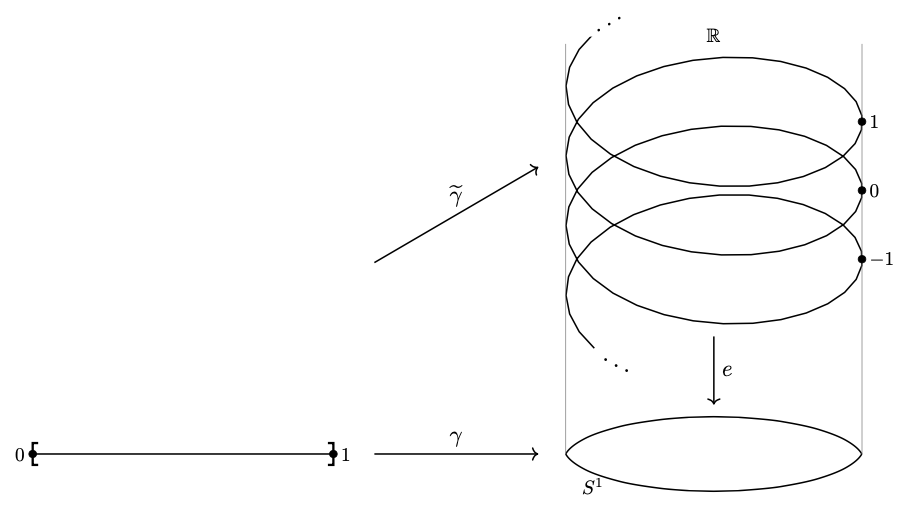
\includegraphics[scale = 0.5]{fotos_topo_2/otrasfotos/elevaciocamins.png}
\end{equation}
Queda provat així que podem construir una aplicació contínua $\overline{\gamma}:I_1\cup\cdots\cup I_n = I\rightarrow\mathbb{R}$ que satisfà $\overline{\gamma}(0)=0$ i $e\circ\overline{\gamma} = \gamma$ partint d'un camí $\gamma:I\rightarrow S^1$ tal que $\gamma(0) = 1$. 

Veurem per acabar que aquesta aplicació $\overline{\gamma}$ és l'única amb les característiques aquí esmentades. Considerem una altra aplicació $\overline{\gamma}':I\rightarrow\mathbb{R}$ amb les mateixes propietats que $\overline{\gamma}$. Així, tindrem, en particular, $e\circ\overline{\gamma}'=\gamma=e\circ\overline{\gamma}$, d'on, per la periodicitat de $e$, cal que la imatge de $I$ per $\overline{\gamma}'-\overline{\gamma}$ sigui un subconjunt de $\mathbb{Z}$. A més, aquest subconjunt ha de ser connex, ja que és la imatge d'un espai connex $I$ per una aplicació contínua $\overline{\gamma}'-\overline{\gamma}$. Ara bé, els únics subconjunts connexos (no buits) de $\mathbb{Z}$ són els conjunts que contenen un sol punt, de manera que $\overline{\gamma}'-\overline{\gamma}$ cal que sigui una aplicació constat. D'aquí sabent que $\overline{\gamma}'(0)-\overline{\gamma}(0) = 0-0=0$ es desprèn $\overline{\gamma}' = \overline{\gamma}$.
\end{proof}

La imatge d'aquesta demostració és la que va proporcionar l'estudiant \textsc{Marí Jané Ballarín} (veure nota del principi de la secció).


\begin{defi}
[Elevació de camins]\label{def:elevaciodecamins}\index{Elevació de camins} Donat un camí continu $\gamma:I\rightarrow S^1$ amb punt base $1\in S^1$, i.e., tal que $\gamma(0) = \gamma(1)=1$, anomenem \textit{elevació de $\gamma$} a una aplicació $\overline{\gamma}:I\rightarrow\mathbb{R}$ que satisfà $e\circ\overline{\gamma} = \gamma$.
\end{defi}

Observem que, en particular, si $\overline{\gamma}$ és l'elevació de $\gamma$ tindrem
\begin{equation}
    \notag
    (e\circ\overline{\gamma})(1)=\gamma(1) = 1\Longrightarrow e^{2\pi i\overline{\gamma}(1)} = 1\Longrightarrow \overline{\gamma}(1)\in\mathbb{Z}.
\end{equation}

\begin{defi}
[Grau d'un camí]\label{def:graudecami}\index{Grau d'un camí} Definim el grau del camí $\gamma:I\rightarrow S^1$ com $\mathrm{gr}(\gamma):=\overline{\gamma}(1)$.
\end{defi}



\begin{ej}
\label{ej:elevaciodecami} L'aplicació $\overline{\gamma}(t) = t$, per tot $t\in I$, és una elevació del camí $\gamma(t) = (e\circ\overline{\gamma})(t)=e^{2\pi it},\;\forall t\in I$, de manera que $\mathrm{gr}(\gamma) = \overline{\gamma}(1) = 1$. De fet, és prou evident que, en general, $\overline{\gamma}_n(t) = nt$ és una elevació de $\gamma_n(t) = e^{2\pi int}\;\forall n\geq 1$ i, per tant, $\mathrm{gr}(\gamma_n) = \overline{\gamma}_n(1) = n$, $\forall n\geq 1$.
\end{ej}

Aquesta definició es pot estendre a tot camí $\gamma$ tancat de $S^1$: podem definir una elevació $\overline{\gamma}$ (no única) d'un tal camí com una aplicació $\overline{\gamma}:I\rightarrow\mathbb{R}$ que verifica $\overline{\gamma}(0)\in e^{-1}(\{\gamma(0)\})$ i $e\circ \overline{\gamma}=\gamma$, i el grau de $\gamma$ com $\mathrm{gr}(\gamma)=\overline{\gamma}(1)-\overline{\gamma}(0)\in\mathbb{Z}$.

És trivial que el lema d'elevació (\ref{lema:elevaciodecamins}) prova que tals aplicacions $\overline{\gamma}$ existeixen. Per construir-ne una tan sols cal seguir els mateixos passos que en aquest resultat, sense la limitació en la tria de l'interval $J_0$ que contingui un element de l'antiimatge de $\gamma(0)$ per $e$; aquesta llibertat és el que fa perdre la unicitat d'elevació. Malgrat això, fixades dues elevacions de $\gamma$, usant els mateixos raonaments que tanquen el lema d'elevació, la seva diferència ha de ser constant i entera. En particular, el grau de $\gamma$ està ben definit, i.e. no depèn de l'elevació que n'haguem escollit, ja que fixades dues elevacions $\overline{\gamma}_1$ i $\overline{\gamma}_2$ de $\gamma$, podent trobar $k\in\mathbb{Z}$ tal que $\overline{\gamma}_1(t) = \overline{\gamma}_2(t) + k$, $\forall t\in I$, tenim que
\begin{equation}
    \notag
    \overline{\gamma}_1(1)-\overline{\gamma}_1(0) = (\overline{\gamma}_2(1)+k) - (\overline{\gamma}_2(0)+k) = \overline{\gamma}_2(1)-\overline{\gamma}_2(0)
\end{equation}

El grau d'un camí, com suggereixen els exemples donats, es correspon amb la idea de quantes voltes complertes fa aquest a $S^1$. Així, seguint de com encetàvem aquest apartat, aquesta aplicació definirà l'isomorfisme entre $\pi(S^1,1)$ i $\mathbb{Z}$ que busquem. Abans, però, haurem de garantir que el grau de dos camins homòtops és el mateix. I per això caldrà generalitzar el concepte d'elevació a les homotopies d'aplicacions.

\begin{lema}
[Elevació d'homotopies]\label{lema:elevaciohomotopies}\index{Lema d'elevació d'homotopies} Per tota aplicació contínua $H:I\times I\rightarrow S^1$ tal que $H(0,s)=1$ $\forall s\in I$ existeix una única nova aplicació contínua $\Tilde{H}:I\times I\rightarrow\mathbb{R}$ tal que $\Tilde{H}(0,s)=0$ $\forall s\in I$ i $e\circ \Tilde{H} = H$.
\end{lema}
\begin{proof}
Considerem, per cada $s\in I$, el camí $H_s(t) = H(t,s)$ que, per hipòtesi, té un punt base 1. Pel lema d'elevació de camins, cada $H_s$ admet una única aplicació $\Tilde{H}_s:I\rightarrow \mathbb{R}$ tal que $e\circ\Tilde{H}_s= H_s$ i $\Tilde{H}_s(0) = 0$. Llavors, és clar que l'aplicació
\begin{equation}
    \notag
    \begin{array}{rl}
        \Tilde{H}:I\times I & \longrightarrow\mathbb{R} \\
        (t,s) & \longmapsto\Tilde{H}_s(t)
    \end{array}
\end{equation}
és l'única que satisfà $e(\Tilde{H}(t,s)) = e(\Tilde{H}_s(t)) = H_s(t)=H(t,s)\;\forall (t,s)\in I\times I$ alhora que $\Tilde{H}(0,s) = \Tilde{H}_s(0) = 0$, $\forall s\in I$.

Vist això, tan sols queda provar que $\Tilde{H}$ és contínua. Per fer-ho, veurem que $\Tilde{H}$ és contínua en un punt arbitrari $(a,b)\in I\times I$. Notem, per començar, que essent $H$ contínua en un compacte com $I\times I$, llavors és uniformement contínua (això és d'Anàlisi Matemàtica). Així podem prendre un cert $\delta >0$ pel qual donats $(x_1,y_1),(x_2,y_2)\in I\times I$ tals que $\|(x_2,y_2)-(x_1,y_1)\|<\delta$, tenim $d_{S^1}(H(x_2,y_2),H(x_1,y_1))<1$, on $d_{S^1}$ denota la mètrica de $S^1$ definida com la longitud del menor dels arcs que uneixen dos punts dins la circumferència. A més, podem suposar que el valor $\delta$ pres és prou petit com per aplicar el lema del nombre de Lebesgue (\ref{lema:nombredelebesgue}) a $I\times I$. Llavors, de manera anàloga que a la prova del lema d'elevació de camins (\ref{lema:elevaciodecamins}) per cada subconjunt $C$ de $I\times I$ de diàmetre menor que $\delta$, tindrem $H(C)\subset U_z$ per un cert $z\in S^1$.

En particular, si $\{t_i\}_{0\leq i\leq n}$ és una successió creixent de nombres tals que $t_0=0$, $t_n=1$ i $|t_i-t_{i-1}|<\delta/2$, $\forall i\in\{1,\ldots,n\}$, els rectangles $R_i = [t_{i-1},t_i]\times [b-\delta/4,b+\delta/4]\subset I\times I$ satisfan la propietat anterior $\forall i\in\{1,\ldots,n\}$. En efecte,
\begin{equation}
    \notag
    \mathrm{diam}(R_i) = \sqrt{(t_i-t_{i-1})^2+(\delta/2)^2}<\sqrt{(\delta/2)^2+(\delta/2)^2} = \frac{\sqrt{2}}{2}\delta<\delta.
\end{equation}
Naturalment, $(a,b)\in R_i$ per un cert $i\in \{1,\ldots,n\}$. Per provar la continuïtat de $\Tilde{H}$ en aquest punt, construirem una funció contínua $\hat{H}$ a $R_1\cup\cdots\cup R_n$ que coincidirà amb la definició de $\Tilde{H}$. En primer lloc, treballant un cop més de manera anàloga a com vam fer a la demostració del lema d'elevació de camins, siguin $z_1\in S^1$ tal que $H(R_1) \subset U_{z_1}$ i $J_1$ l'interval de $e^{-1}(U_{z_1})$ que conté $0\in \mathbb{R}$. Podem assegurar que aquest últim interval existeix ja que cal $H(0,b) = 1\in U_{z_1}=S^1\setminus\{z_1\}$ i.e. $z_1\not=1$. D'aquí, com que $e$ restringida a $J_1$ és un homeomorfisme, podem definir $\hat{H}$ a $R_1$ com $\hat{H}_{|R_1} = (e_{|J_1})^{-1}\circ H_{|R_1}$, de manera que és clarament contínua. A més a més, trivialment, $\hat{H}_{|R_1}$ satisfà $e\circ \Tilde{H}_{|R_1} = H_{|R_1}$ i $\hat{H}_{|R_1}=\Tilde{H}_{|R_1}$.

A partir d'aquí és qüestió d'estendre la definició de $\hat{H}$ a $R_1\cup \cdots \cup R_n$ de manera que coincideixi amb la de $\Tilde{H}$ i sigui contínua. Novament, això ho farem per inducció. Concretament, suposant que $\hat{H}$ és definida contínua a $P_i = R_1\cup\cdots\cup R_i$ i satisfà $e\circ \hat{H}_{|P_i}=H_{|P_i}$ per un cert $i\in\{1,\ldots,n-1\}$, siguin $z_{i+1}\in S^1$ tal que $H(R_{i+1})\subset U_{z_{i+1}}$ i $J_{i+1}$ l'interval de $e^{-1}(U_{z_{i+1}})$ que conté $\hat{H}(t_i,s)$ $\forall s\in [b-\delta/4,b+\delta/4]$. Notem que tal interval existeix ja que, com que $(t_i,s)\in R_i\cap R_{i+1}$ $\forall s\in [b-\delta/4,b+\delta/4]$, llavors $(e\circ \hat{H})(t_i,s) = H(t_i,s)\in U_{z_{i+1}}$ d'on, per la continuïtat de $\hat{H}$ en $R_i$ cal que tot $\hat{H}(t_i,s)$ amb $s\in [b-\delta/4,b+\delta/4]$ pertanyi una mateixa component connexa de $e^{-1}(U_{z_{i+1}})$. Així, podem estendre $\hat{H}$ a $P_{i+1}$ definit $\hat{H}_{|R_{i+1}} = (e_{|J_{i+1}})^{-1}\circ H_{|R_{i+1}}$, de manera que hi serà contínua i es complirà trivialment $e\circ \hat{H}_{|P_{i+1}} = H_{|P_{i+1}}$.

Queda provat així que podem construir una aplicació contínua $\hat{H}:P_n = R_1\cup\cdots\cup R_n\rightarrow\mathbb{R}$ que satisfà $e\circ \hat{H} = H_{|P_n}$ i $\hat{H}(0,s) = s$ $\forall s\in[b-\delta/4,b+\delta/4]$. Havent vist que l'única aplicació amb aquestes propietats és $\Tilde{H}$, cal $\hat{H} = \Tilde{H}_{|P_n}$, d'on $\Tilde{H}$ és contínua a $P_n$. En particular, ho és a $(a,b)$.
\end{proof}


\begin{ter}
[Grup fonamental de la circumferència]\label{ter:grupfonamentalcircumferencia}\index{Teorema del grup fonamental de la circumferència}
\end{ter}
\begin{proof}
L'aplicació
\begin{equation}
    \notag
    \begin{array}{rl}
        \mathrm{Gr}:\pi(S^1,1) & \longrightarrow\mathbb{Z} \\
        \left[\gamma\right] & \longmapsto \mathrm{gr}(\gamma)
    \end{array}
\end{equation}
és un isomorfisme de grups i, per tant, $\pi(S^1,1)\cong \mathbb{Z}$.
\end{proof}
\begin{proof}
Com hem insinuat en presentar el lema anterior, el primer que cal veure és, naturalment, que l'aplicació Gr està ben definida. A continuació, caldrà provar que és un morfisme de grups i, per últim, que aquest morfisme és bijectiu.
\begin{itemize}
    \item \underline{Ben definida}. Per començar hem de provar que donats dos camins $\gamma_0,\gamma_1$ de $S^1$ amb punt base 1 i homòtops entre ells compleixen $\mathrm{gr}(\gamma_0) = \mathrm{gr}(\gamma_1)$. Considerem per això una homotopia $H$ entre aquests dos camins. Pel lema d'elevació d'homotopies (\ref{lema:elevaciohomotopies}), podem prendre $\Tilde{H}:I\times I\rightarrow\mathbb{R}$ contínua i tal que $e\circ \Tilde{H} = H$ i $\Tilde{H}(0,t) = 0$, $\forall t\in I$. A partir d'aquesta podem definir també els camins $\Tilde{\gamma}_0(t) = \Tilde{H}(t,0)$ i $\Tilde{\gamma}_1(t) = \Tilde{H}(t,1)$ $\forall t\in I$. És prou fàcil veure que aquests camins són elevacions de $\gamma_0$ i $\gamma_1$, respectivament; per una banda, per construcció de $\Tilde{H}$, és clar que $\Tilde{\gamma}_0(0) = 0 = \Tilde{\gamma}_1(0)$ i, per l'altra banda
    \begin{equation}
        \notag
        (e\circ\Tilde{\gamma}_i)(t) = (e\circ \Tilde{H})(t,i) = H(t,i) = \gamma_i(t) \;\forall t\in I,\;i\in\{0,1\}
    \end{equation}
    Ara, essent $H$ una homotopia d'extrems fixos (veure definició d'homotopia de camins (\ref{def:homotopiadecamins})), se satisfà $(e\circ \Tilde{H})(1,s) = H(1,s) = \gamma_0(1)=1\;\forall s\in I$. Dit d'una altra manera, es compleix $e^{2\pi i\Tilde{H}(1,s)} = 1$, d'on $\Tilde{H}(1,s)\in\mathbb{Z}\;\forall s\in I$. Així, com que $\Tilde{H}(1,\cdotp)$ és una aplicació contínua amb espai de sortida connex $I$, la seva imatge ha de ser un subconjunt connex de $\mathbb{Z}$, cosa que ens porta a concloure que $\Tilde{H}(1,\cdotp)$ és constant. Per tant,
    \begin{equation}
        \notag
        \mathrm{gr}(\gamma_0)= \Tilde{\gamma}_0(1) = \Tilde{H}(1,0) = \Tilde{H}(1,1) = \Tilde{\gamma}_1(1) = \mathrm{gr}(\gamma_1)
    \end{equation}
    
    \item \underline{Morfisme de grups}. Partint dels camins arbitraris $\gamma_0$ i $\gamma_1$ com abans, veurem que $\mathrm{Gr}([\gamma_0][\gamma_1]) = \mathrm{Gr}([\gamma_0]) + \mathrm{Gr}([\gamma_1])$. Recuperant les elevacions $\Tilde{\gamma}_0$ i $\Tilde{\gamma}_1$ d'aquests camins, tindrem que
    \begin{equation}
        \notag
        (\gamma_0*\gamma_1)(t) =\left\{
        \begin{array}{ll}
            \gamma_0(2t) & \mathrm{si}\;t\in[0,1/2] \\
            \gamma_1(2t-1) & \mathrm{si}\;t\in[1/2,1]
        \end{array}
        \right.
        =
        \left\{
        \begin{array}{ll}
            e^{2\pi i\Tilde{\gamma}_0(2t)} & \mathrm{si}\;t\in[0,1/2] \\
            e^{2\pi i\tilde{\gamma}_1(2t-1)} & \mathrm{si}\;t\in[1/2,1]
        \end{array}
        \right.
    \end{equation}
    Així, si $\gamma = \gamma_0*\gamma_1$, llavors
    \begin{equation}
        \notag
        \tilde{\gamma}(t) = \left\{
        \begin{array}{rl}
            \tilde{\gamma}_0(2t) & \mathrm{si}\;t\in[0,1/2] \\
            \tilde{\gamma}_1(2t-1) & \mathrm{si}\;t\in[1/2,1]
        \end{array}
        \right.
    \end{equation}
    és una elevació de $\gamma$. Cal demostrar que això és cert.
    
    En primer lloc, com que, atès que $\tilde{\gamma}_0(0) = 0 = \tilde{\gamma}_1(0)$ per ser $\tilde{\gamma}_0$ i $\tilde{\gamma}_1$ elevacions de $\gamma_0$ i $\gamma_1$ respectivament, tenim que $\tilde{\gamma}(0) = \tilde{\gamma}_0(2\cdotp 0) = \tilde{\gamma}_0(0) = 0$. De manera simètrica, veiem que $\tilde{\gamma}$ és una aplicació contínua: ho és en tot $t\in I\setminus\{1/2\}$ de manera trivial ja que és definida en termes de les aplicacions contínues $\tilde{\gamma}_0,\tilde{\gamma}_1$, i també ho és en $t = 1/2$, ja que
    \begin{equation}
        \notag
        \left.
        \begin{array}{ll}
            \tilde{\gamma}_0(2\cdotp\frac{1}{2}) = \tilde{\gamma}_0(1) \\
            \tilde{\gamma}_1(2\cdotp\frac{1}{2}-1)+\tilde{\gamma}_0(1) = \tilde{\gamma}_1(0)-\tilde{\gamma}_0(1) = \tilde{\gamma}_0(1)
        \end{array}
        \right\} \Rightarrow \tilde{\gamma}(1/2) := \tilde{\gamma}_0(1)
    \end{equation}
    Per acabar, tenim en compte que $\tilde{\gamma}_0(1) = \mathrm{gr}(\gamma_1)\in\mathbb{Z}$ i, per tant, $e^{2\pi i\tilde{\gamma}_0(1)}=1$, l'aplicació $\tilde{\gamma}$ compleix
    \begin{equation}
        \notag
        (e\circ\tilde{\gamma})(t) = \left\{
        \begin{array}{rl}
            e^{2\pi i\Tilde{\gamma}_0(2t)} & \mathrm{si}\;t\in[0,1/2] \\
            e^{2\pi i(\tilde{\gamma}_1(2t-1)+\tilde{\gamma}_0(1)} & \mathrm{si}\;t\in[1/2,1]
        \end{array}
        \right. = 
        \left\{
        \begin{array}{rl}
            e^{2\pi i\Tilde{\gamma}_0(2t)} & \mathrm{si}\;t\in[0,1/2] \\
            e^{2\pi i\tilde{\gamma}_1(2t-1)}e^{2\pi i(\tilde{\gamma}_0(1)} & \mathrm{si}\;t\in[1/2,1]
        \end{array}
        \right.
    \end{equation}
    En altres paraules, $e\circ\tilde{\gamma}=\gamma$. Amb tot obtenim
    \begin{equation}
        \notag
        \mathrm{Gr}([\gamma_0][\gamma_1]) = \mathrm{Gr}([\gamma_0*\gamma_1]) = \mathrm{Gr}([\gamma]) = \mathrm{gr}(\gamma) = \tilde{\gamma}(1) = 
    \end{equation}
    \begin{equation}
        \notag
        = \tilde{\gamma}_1(1)+\tilde{\gamma}_0(1) = \mathrm{gr}(\gamma_1)+\mathrm{gr}(\gamma_0) =\mathrm{Gr}([\gamma_1])+\mathrm{Gr}([\gamma_0])
    \end{equation}
    
    
    \item \underline{Morfisme bijectiu}. Tan sols falta veure que el morfisme $\mathrm{Gr}$ és bijectiu. Per a la seva exhaustivitat recordem els exemples vistos d'elevacions de camins (\ref{ej:elevaciodecami}), on vèiem que el camí $\gamma_n(t) = e^{2\pi int}$ té grau $n\in\mathbb{Z}$ per tot $n$; pel que fa a la injectivitat de Gr serà suficient veure que $\mathrm{Gr}([\gamma]) = \mathrm{gr}(\gamma) = 0$ si i només si $[\gamma] = [\delta_1]$, i.e. $\gamma\sim \delta_1$, on $\delta_1$ és el camí constant igual a $1\in S^1$. Notem que en tal cas, l'elevació $\tilde{\gamma}$ de $\gamma$ complirà $\tilde{\gamma}(0) = 0 = \mathrm{gr}(\gamma) = \tilde{\gamma}$; en definitiva, tindrem que $\tilde{\gamma}$ és un camí tancat en $\mathbb{R}$ amb punt base 0. Recordem, de (\ref{ej:grupfonamentalder}) que $\pi(\mathbb{R},0) = \{[\varepsilon_0]\} = \{\mathrm{id}\}$, on $\varepsilon$ és el camí constant igual a 0, de manera que $\tilde{\gamma}$ i $\varepsilon_0$ són homòtops. D'aquí, prenent una homotopia $G$ entre $\tilde{\gamma}$ i $\varepsilon_0$, essent $e:\mathbb{R}\rightarrow S^1$ una aplicació contínua per les propietats que relacionen tals aplicacions amb les homotopies vistes anteriorment, l'aplicació $e\circ G$ defineix una homotopia entre els camins $e\circ\tilde{\gamma} = \gamma$ i $e\circ\varepsilon_0 = \delta_1$, que és el que volíem.
\end{itemize}
\end{proof}







A continuació, calcularem el grup fonamental d'altres coneguts espais topològics, així com el tor o el pla projectiu. Aquests exemples són extrets de \cite{topologiaparausuarios} i de \cite{mathonline}. 

\begin{ej}
[Grup fonamental del tor] Podem utilitzar el resultat de (\ref{exercici2.5.ab}) per concloure que el tor té grup fonamental:
\begin{equation}
    \notag
    \pi(\mathbb{T}, (x,y)) \cong \pi(S^1\times S^1, (x,y)) \cong \pi(S^1,x)\times \pi(S^1,y)\cong \mathbb{Z}\times\mathbb{Z}.
\end{equation}
\end{ej}

\begin{ej}
[Grup fonamental del cilindre] Pensant el cilindre com el producte $S^1\times I$, on $I=[0,1]\subset\mathbb{R}$. Per tant, el grup fonamental és $\pi(S^1)\times \pi(I)$, però $\pi(S^1) \cong \mathbb{Z}$ i $\pi(I)\cong \{\mathrm{id}\}$. Per tant, el grup fonamental del cilindre és isomorf a $\mathbb{Z}\times\{\mathrm{id}\}\cong \mathbb{Z}$.
\end{ej}










\section{Aplicacions del grup fonamental a la topologia del pla}

Els conceptes i resultats vistos fins ara permeten provar propietats de les funcions del pla que tenen algunes aplicacions remarcables.

\subsection{Teorema del punt fix de Brouwer}


\begin{defi}
[Propietat del punt fix]\label{def:propietatdelpuntfix}\index{Propietat del punt fix} Un espai $X$ té la \textit{propietat del punt fix} si per a tota aplicació contínua $f:X\rightarrow X$, existeix algun punt fix $p\in X$ tal que $f(p) = p$.
\end{defi}


\begin{ter}
[Teorema del punt fix de Brouwer]\label{ter:puntfixbrouwer}\index{Teorema del punt fix de Brouwer} Tota aplicació contínua $f:D^2\rightarrow D^2$, on $D^2$ és el disc unitat, $D^2 = \{(x,y)\in\mathbb{R}^2\;:\;x^2+y^2\leq 1\}$, té un punt fix, i.e. $\exists p\in D^2$ tal que $f(p) = p$.
\end{ter}
\begin{proof}
Suposem que, per contra, $f(p) \not=p$, $\forall p\in D^2$ i busquem arribar a una contradicció.

Considerem per començar l'aplicació $r:D^2\rightarrow S^1$ que envia cada punt $p\in D^2$ a la intersecció amb la semirecta que surt de $f(p)\in D^2$ i passa per $p$.

És evident que $r$ està ben definida ja que no tenint $f$ punts fixos, sempre existeix la semirecta que ens ocupa. Es pot veure, a més, que aquesta aplicació és contínua.

Com són els punts de les imatges? Veiem que són de la forma $f(p) + t(p-f(p))$, amb $t\geq 0$. D'aquesta manera, d'entre aquests valors, $r(p)$ pren l'únic $\lambda(p)\geq 0$ que satisfà $\|f(p)+\lambda(p)(p-f(p))\|^2 = 1$ (perquè ha de caure a $S^1$ i per tant el mòdul ha de ser 1).

Considerem el polinomi $P(t) = \|f(p)+t(p-f(p))\|^2-1$. Naturalment $\lambda(p)$ serà una arrel d'aquest plinomi. Veurem que aquest polinomi només admet una arrel positiva, cosa que ens assegurarà que $\lambda$ està ben definida i és contínua, ja que ve donada com a transformacions contínues dels coeficients de $P(t)$, que són en sí funcions contínues de $p$. 

Utilitzant el criteri de signes de Descartes podem observar que el coeficient dominant de $P(t)$ és estrictament positiu (perquè és una norma i per hipòtesi $f(p) \not=p\;\forall p\in D^2$). Llavors, hi haurà només un canvi de signe en els coeficients de $P$ ordenats decreixentment per grau, cosa que demostra que $P$ té una única arrel positiva, definida per $\lambda$ i, de retruc, la continuïtat de $r$.

Per altra banda, és fàcil veure que, per construcció, $r_{|S^1} = \mathrm{id}_{|S^1}$, d'on $r$ és una retracció de $S^1$ en $D^2$. Veurem, però, que $S^1$ no és un retracte de $D^2$. En efecte, si $i:S^1\hookrightarrow D^2$ és la inclusió, essent $i$ i $r$ contínues, tenim que
\begin{equation}
    \notag
    r_*\circ i_* = (r\circ i)_* = (\mathrm{id}_{S^1})_* = \mathrm{id}_{\pi(S^1,1)}
\end{equation}
cosa que no pot ser ja que $\pi(D^2,1)\cong \{\mathrm{id}\}$ mentre hem vist abans que $\pi(S^1,1)\cong\mathbb{Z}$, impossibilitant que $r_*$ retorni $\mathrm{id}\in \pi(D^2,1)$ a cada element de $\pi(S^1,1)$. Aquesta contradicció amb què hem topat prové de suposar que $f$ no té punts fixos, de manera que concloem que existeix algun punt fix.
\end{proof}

\begin{coro}
\label{coro:puntfixbrouwer} Si $X$ és homeomorf a $D^2$, llavors tota aplicació contínua $g:X\rightarrow X$ té un punt fix.
\end{coro}
\begin{proof}
Sigui $h$ un homeomorfisme entre $X$ i $D^2$, de manera que, donada una aplicació contínua $g:X\rightarrow X$, la composició $f = h\circ g\circ h^{-1}$ és una aplicació contínua de $D^2$ en sí mateix. Així doncs, pel teorema del punt fix de Brouwer, $\exists q\in D^2$ tal que $f(q) = (h\circ g\circ h^{-1})(q) = q$, d'on $(g\circ h^{-1})(q) = h^{-1}(q)$ i.e. $h^{-1}(q)\in X$ és un punt fix per $g$.
\end{proof}

\begin{ej}
[Exercici 17]\label{exercici2.17} Es vol demostrar que el sistema
\begin{equation}
    \notag
    \left\{
    \begin{array}{ll}
        x = \varphi_1(x) = \cos(1+\sin(x^2+y^7)) \\
        y = \varphi_2(x) = \sin(1+\cos(x^7+y^2))
    \end{array}
    \right.
\end{equation}
té alguna solució a $\mathbb{R}^2$. Garantir això és equivalent a mostrar que l'aplicació $\varphi:\mathbb{R}^2\rightarrow\mathbb{R}^2$ definida com $\varphi(x,y) = (\varphi_1(x,y),\varphi_2(x,y))$ té un punt fix. Observem que podem trobar un cert quadrat $Q\subset \mathbb{R}^2$ que contingui la imatge de $\varphi$, ja que les seves components són funcions trigonomètriques acotades. Llavors, com que tot quadrat $Q$ és homeomorf al disc unitat, el teorema del punt fix de Brouwer (i el corol·lari anterior) ens assegura que $\varphi$ té algun punt fix dins de $Q$.
\end{ej}



\begin{prop}
[Exercici 11a]\label{exercici2.11.a} Si un espai $X$ té la propietat del punt fix i $A$ és un retracte de $X$, llavors $A$ també té la propietat del punt fix.
\end{prop}
\begin{proof}
Sigui $f:A\rightarrow A$ una aplicació contínua. Volem demostrar que $\exists p\in A$ tal que $f(p) = p$. Com $A$ és un retracte de $X$, existeix una retracció $r:X\rightarrow A$, de forma que si $i:A\rightarrow X$ és la inclusió, es té que $r\circ i = \mathrm{id}_A$.

Considerem l'aplicació $g:X\rightarrow X$ definida com
\begin{equation}
    \notag
    g= i\circ f\circ r: X\rightarrow A\rightarrow A\rightarrow X.
\end{equation}
Com $X$ té la propietat del punt fix, existeix un $x_0\in X$ tal que $g(x_0) = x_0$, és a dir, $(i\circ f\circ r)(x_0) = x_0$. Com que $\mathrm{Im}(i\circ f)\subseteq A$ es té que $x_0\in A$ i com que $\forall a\in A$, $r(a) = a$, tenim que $r(x_0) = x_0$ Finalment doncs tenim que
\begin{equation}
    \notag
    x_0 = g(x_0) = (i\circ f\circ r)(x_0) = i(f(r(x_0))) = i(f(x_0))
\end{equation}
i això és cert si, i només si, $f(x_0) = x_0$, ja que $x_0\in A$. Per tant $A$ té també la propietat del punt fix.
\end{proof}

\begin{coro}[Exercici 11a]\label{exercici2.11.a.2}
Si $X$ i $Y$ són dos espais topològics tals que $X\times Y$ té la propietat del punt fix, aleshores $X$ i $Y$ també la tenen.
\end{coro}
\begin{proof}
Si el producte $X\times Y$ té la propietat del punt fix, aleshores com que $X\times \{y_0\}\rightarrow X\times Y$ (per $y_0\in Y$) és un retracte de $X\times Y$, tenim que $X\times \{y_0\}$ té la propietat del punt fix. Això és, $X$ té la propietat del punt fix.
\end{proof}

\begin{prop}
[Exercici 11b]\label{exercici2.11.b} La propietat del punt fix es conserva per homeomorfismes.
\end{prop}
\begin{proof}
Si $h:X\rightarrow Y$ és un homeomorfisme i $X$ té la propietat del punt fix, anem a veure que $Y$ també la té. En efecte, sigui $f:Y\rightarrow Y$ una aplicació contínua. Podem considerar
\begin{equation}
    \notag
    g = h^{-1}\circ f\circ h:X\rightarrow Y\rightarrow X
\end{equation}
Aquesta aplicació $g:X\rightarrow X$ té un punt fix (ja que si $X$ té la PPF, aleshores tota aplicació contínua té un punt fix) és a dir, existeix un $x_0\in X$ tal que $g(x_0) = x_0$. Aplicant la definició de $g$ obtenim que
\begin{equation}
    \notag
    h^{-1}\circ f\circ h(x_0) = x_0 \Rightarrow (f\circ h)(x_0) = h(x_0) \Rightarrow f(h(x_0)) = h(x_0)
\end{equation}
i com que $h(x_0)\in Y$, podem anomenar $y_0:=h(x_0)$ i aleshores és un punt fix de $f$. Per tant $Y$ satisfà la propietat del punt fix.
\end{proof}

\begin{nota}
[Exercici 11b]\label{exercici2.11.b.2} La propietat del punt fix no té per què conservar-se per equivalències homotòpiques.
\end{nota}
\begin{proof}
En efecte, si prenem $\mathbb{R}\simeq *$ (que és una equivalència homotòpica ja provada) observem que $*$ té la propietat del punt fix, ja que $f(*) = *$ per a qualsevol aplicació contínua $f:*\rightarrow *$ (ja que $*\in *$ és l'únic element de $*$). Ara bé, $\mathbb{R}$ no té la PPF perquè, per exemple, $\exists$ aplicació contínua $t:\mathbb{R}\rightarrow \mathbb{R}$, $t(x) = x+1$ que no té cap punt fix.
\end{proof}

\begin{ej}
[Exercici 11c]\label{exercici2.11.c} Veiem exemples d'espais topològics que tenen o no tenen la propietat del punt fix, basant-nos en les proposicions anteriors.
\begin{enumerate}[(i)]
    \item $S^n$ no té la propietat del punt fix, ja que, per exemple, l'aplicació antipodal $a:S^n\rightarrow S^n$, $a(x) = -x$, $\forall x\in S^n$, és contínua i no té cap punt fix.
    \item La bola oberta $(B^\circ)^n \subseteq \mathbb{R}^n$ no té la propietat del punt fix ja que és homeomorfa a $\mathbb{R}^n$ i aleshores, per (\ref{exercici2.11.a}), tindrà la PPF si $\mathbb{R}^n$ la té, però $\mathbb{R}^n$ no la té perquè podem considerar l'aplicació $t:\mathbb{R}^n\rightarrow \mathbb{R}^n$, $t(x) =x+v$, amb $v\in\mathbb{R}^n\setminus\{0\}$ fixat, és una aplicació contínua sense cap punt fix.
    \item El tor $T_n = S^1\times\cdots\times S^1$ no té la PPF ja que $S^1$ és un retracte del tor $T_n$ i aplicant el contrarrecíproc de (\ref{exercici2.11.a}) obtenim doncs que, com $S^1$ no té la propietat del punt fix, aleshores $T_n$ tampoc.
    \item El disc tancat $D^2$ sí té la propietat del punt fix: és el Teorema del Punt Fix de Brouwer (\ref{ter:puntfixbrouwer}).
    \item $S^1\vee S^1$ (la unió puntual de dues circumferències) no té la propietat del punt fix, ja que $S^1$ és un retracte de $S^1\vee S^1$ i, de nou, aplicant (\ref{exercici2.11.a}) veiem que no ho compleix. Demostrem, però, que és un retracte: En efecte, considerem $S^1\vee S^1$ (agafem alguna aplicació translació que ens ho mogui de forma que el punt on s'uneixen sigui l'origen de coordenades) i definim l'aplicació
    \begin{equation}
        \notag
        r(x) = \left\{
        \begin{array}{ll}
            x & \mathrm{si}\;x=(x,y),\;x>0 \\
            (0,0) & \mathrm{si}\;x=(x,y),\;x\leq 0
        \end{array}
        \right.
    \end{equation}
    És immediat que $r$ és contínua i que $r$ és una retracció $S^1\vee S^1\rightarrow S^1$.
    \item $D^2\vee D^2$ (la unió puntual de dos discs tancats) sí que té la propietat del punt fix, ja que és un retracte de $D^2$ i $D^2$ hem dit que pel Teorema del Punt Fix de Brouwer tenia la PPF.
\end{enumerate}
\end{ej}



\subsection{Índex d'un camí tancat al pla respecte un punt}

El que volem fer ara és demostrar el teorema de Bolzano en $\mathbb{R}^2$ però per poder fer-ho ens falten encara algunes nocions prèvies en la topologia del pla.

El següent resultat que provarem és l'anàleg del Teorema de Bolzano per a funcions de $\mathbb{R}^2$ en $\mathbb{R}^2$. Recordem com era el teorema de Bolzano:
\begin{ter}
[Teorema de Bolzano]\label{ter:bolzano}\index{Teorema de Bolzano} Donada una funció contínua $f:D^1=[-1,1]\rightarrow\mathbb{R}$, per cada $q\in[f(-1),f(1)]$ podem trobar $p\in [-1,1]$ tal que $f(p) = q$.
\end{ter}

En essència, tenint en compte que $S^0 = \partial D^1 = \{-1,1\}$, estem dient que si $q\in \mathbb{R}$ està ``envoltat'' per la imatge de $S^0$ per $f$, llavors $q\in f(D^1)$. A continuació provarem el mateix per a dimensió 2. Abans, però, cal definir la noció intuïtiva d'estar ``envoltat''.

\begin{nota}
Sempre que convingui identificarem el pla $\mathbb{R}^2$ amb el cos dels complexos $\mathbb{C}$. Aleshores tot camí tancat $\sigma:I\rightarrow \mathbb{R}^2$ es pot interpretar com una aplicació $\hat{\sigma}:S^1\rightarrow \mathbb{R}^2$ tal que $\sigma(t) = \hat{\sigma}(e^{2\pi it}$.
\end{nota}

\begin{defi}
[Camí tancat associat]\label{def:camitancatassociat}\index{Camí tancat associat a una aplicació} Partint d'una funció contínua $f:S^1\rightarrow S^1$, podem associar-li el camí tancat
\begin{equation}
    \notag
    \begin{array}{rl}
        \gamma_f:I & \longrightarrow S^1 \\
        t & \longmapsto f(e^{2\pi it})
    \end{array}
\end{equation}
    que satisfà $\gamma_f = f\circ e$.
\end{defi}

Aquest camí, encara que sigui tancat, no té necessàriament punt base $1\in S^1$. Sempre podem prendre, però, el camí $\hat{\gamma}_f:I\rightarrow S^1$ definit com 
\begin{equation}
    \notag
    \hat{\gamma}_f(t) = \frac{\gamma(f)}{f(1)}=\frac{f(e^{2\pi it)}}{f(1)}\quad \forall t\in I,
\end{equation}
que sí que té 1 com a punt base.

\begin{prop}
\label{prop:funcionscaminshomotops} Donades dues funcions contínues $f,g:S^1\rightarrow S^1$, es compleix $f\simeq g$ si, i només si, com a camins, $\hat{\gamma}_f\simeq \hat{\gamma}_g$.
\end{prop}
\begin{proof}
Veiem cada implicació:
\begin{enumerate}[($\Rightarrow$)]
    \item Fixem una homotopia $G:S^1\times I\rightarrow S^1$ entre $f$ i $g$. És prou fàcil comprovar que l'aplicació
    \begin{equation}
        \notag
        \begin{array}{rl}
            \tilde{G}:I\times I & \longrightarrow S^1 \\
            (t,s) & \longmapsto \tilde{G}(t,s):=\dfrac{G(e^{2\pi it},s)}{G(1,s)},
        \end{array}
    \end{equation}
    que està ben definida ja que, per hipòtesi, $G(z,s)\in S^1$, $\forall (z,s)\in S^1\times I$, és una homotopia entre els camins $\hat{\gamma}_f$ i $\hat{\gamma}_g$. En efecte, per les propietats de la homotopia d'aplicacions $G$ (veure \ref{def:homotopia}), tenim que $\tilde{G}$ és contínua i
    \begin{equation}
        \notag
        \tilde{G}(t,0) = \frac{G(e^{2\pi it},0)}{G(1,0)} = \frac{f(e^{2\pi it})}{f(1)} = \hat{\gamma}_f(t)\quad\forall t\in I
    \end{equation}
    i, de manera anàloga,
    \begin{equation}
        \notag
        \tilde{G}(t,1) = \frac{G(e^{2\pi it},1)}{G(1,1)} = \frac{f(e^{2\pi it})}{g(1)} = \hat{\gamma}_g(t)\quad \forall t\in I.
    \end{equation}
    A més, $\tilde{G}$ manté els extrems fixos:
    \begin{equation}
        \notag
        \tilde{G}(0,s) = \frac{G(e^{2\pi i\cdotp 0},s)}{G(1,s)} = \frac{G(1,s)}{G(1,s)} = 1 = \hat{\gamma}_f(0) = \hat{\gamma}_g(0)\quad \forall s\in I
    \end{equation}
    \begin{equation}
        \notag
        \tilde{G}(1,s) = \frac{G(e^{2\pi i\cdotp 1},s)}{G(1,s)} = \frac{G(1,s)}{G(1,s)} = 1 = \hat{\gamma}_f(1) = \hat{\gamma}_g(1)\quad \forall s\in I
    \end{equation}
\end{enumerate}
\begin{enumerate}[($\Leftarrow$)]
    \item Donada una homotopia $H$ entre $\hat{\gamma}_f$ i $\hat{\gamma}_g$, considerem l'aplicació $\tilde{H}(z,s) = H(\frac{\arg z}{2\pi},s)$, on $\arg z$ és la branca de l'argument que pren imatges a l'interval $(0,2\pi)$ i satisfà $\arg(-1) = \pi$. Així definida, aquesta aplicació no pot ser una homotopia ja que no és contínua:; cap branca de l'argument pot ser-ho en $S^1$, com es veu a l'assignatura d'Anàlisi Complexa.
    
    Ara bé, tenint en compte que $H$ és una homotopia de camins (veure \ref{def:homotopiadecamins}), en particular, tenint en compte que $\hat{\gamma}_f$ i $\hat{\gamma}_g$ són camins amb punt base $1\in S^1$, satisfà $H(0,s) = 1 = H(1,s) = H(\frac{2\pi}{2\pi},s)$, $\forall s\in I$. Així, si estenem la definició de $\tilde{H}$ a 
    \begin{equation}
        \notag
        \begin{array}{rl}
            \tilde{H}:S^1\times I & \longrightarrow S^1 \\
            (z,s) & \longmapsto \left\{
            \begin{array}{ll}
                1 & \mathrm{si}\;z=1 \\
                H\left(\frac{\arg z}{2\pi},s\right) & \mathrm{altrament}
            \end{array}
            \right.
        \end{array}
    \end{equation}
    ara sí que és una aplicació contínua (prenent la mateixa determinació de l'argument d'abans). Observem, a més, que $\tilde{H}$ és una homotopia entre les funcions $\hat{f},\hat{g}:S^1\rightarrow S^1$ definides com $\hat{f}(z) = \frac{f(z)}{f(1)}$ i $\hat{g}(z) = \frac{g(z)}{g(1)}$, $\forall z\in S^1$, ja que
    \begin{equation}
        \notag
        \tilde{H}(z,0) = H\left(\frac{\arg z}{2\pi},0\right) = \hat{\gamma}_f\left(\frac{\arg z}{2\pi}\right)=\frac{f(e^{2\pi\cdotp\frac{\arg z}{2\pi}})}{f(1)} = \frac{f(e^{i\arg z})}{f(1)} = \hat{f}(z)
    \end{equation}
    per tot $z\in S^1\setminus\{1\}$. I si $z = 1$ també es troba que $\tilde{H}(1,0) = 1 = \frac{f(1)}{f(1)} = \tilde{f}(1)$. Es veu de manera anàloga que $\tilde{H}(z,1) = \hat{g}(z)$, $\forall z\in S^1$.
    
    Ara, però, amb això hem demostrat que si $\hat{\gamma}_f\simeq \hat{\gamma}_g$ aleshores $\hat{f}\simeq \hat{g}$. Faltarà provar que $\hat{f}\simeq f$ i $\hat{g}\simeq g$ de manera que per la transitivitat de la relació d'homotopia (\ref{exercici1.1}), tindrem $f\simeq g$.
    
    Fixat $\zeta\in [0,2\pi)$ tal que $f(1) = e^{i\theta}\in S^1$, valor que existeix i està ben definit ja que $e$ és bijectiva en $[0,2\pi)$, serà suficient observar que l'aplicació $\hat{H}:S^1\times I\rightarrow S^1$ definida com $\hat{H}(z,s) =\frac{f(z)}{e^{i\theta s}}$ $\forall (z,s)\in S^1\times I$, és una homotopia entre $f$ i $\hat{f}$. En efecte, $\hat{H}$ és contínua ja que és quocient de funcions contínues i el seu denominador és no nul (és un element de $S^1$) i satisfà
    \begin{equation}
        \notag
        \hat{H}(z,0) = \frac{f(z)}{e^{i\theta\cdotp 0}} = \frac{f(z)}{1} = f(z),\quad \forall z\in S^1
    \end{equation}
    \begin{equation}
        \notag
        \hat{H}(z,1) = \frac{f(z)}{e^{i\theta\cdotp 1} = \frac{f(z)}{f(1)}} = \hat{f}(z),\quad\forall z\in S^1
    \end{equation}
    i per tant se satisfà el que volíem.
\end{enumerate}
\end{proof}

Després d'aquesta llarga demostració, hem provat que dues aplicacions són homotòpicament equivalents si i només si, els seus camins tancats associats són homotòpicament equivalents com a camins. Vist això, té sentit definir la noció de grau d'una aplicació de $S^1$ en $S^1$.

\begin{defi}
[Grau d'una aplicació de $S^1$ en $S^1$]\label{def:grauaplicacio}\index{Grau d'una aplicació de $S^1$ en $S^1$} Anomenem grau d'una aplicació contínua $f:S^1\rightarrow S^1$ al grau del seu camí (veure \ref{def:graudecami}) associat $\hat{\gamma}_f$. Naturalment, aquest coincidirà amb el grau del camí $\gamma = f\circ e$.
\end{defi}



\begin{defi}
[Classes d'homotopia d'aplicacions de $S^1$ en $S^1$]\label{def:classesdhomotopiadaplicacions}\index{Classes d'homotopia d'aplicacions de $S^1$ en $S^1$} Tenint en compte la relació d'homotopia entre aplicacions, podem definir el conjunt de classes d'homotopia d'aplicacions de $S^1$ en $S^1$, que denotarem com $[S^1,S^1]$. L'operació d'aquest conjunt vindrà definida per $[f]\cdotp[g]:=[fg]$, on $fg:S^1\rightarrow S^1$ és $(fg)(z) = f(z)g(z)$, $\forall z\in S^1$.
\end{defi}

\begin{prop}
\label{prop:productedeclassesdhomotopiadaplicacions} El producte de classes definit com
\begin{equation}
    \notag
    \begin{array}{rl}
        \cdotp:[S^1,S^1]\times [S^1,S^1] & \longrightarrow [S^1,S^1] \\
        ([f],[g]) & \longmapsto [fg]
    \end{array}
\end{equation}
està ben definit, és a dir, no depèn del representant pres de cada classe.
\end{prop}
\begin{proof}
Aquesta proposició és equivalent a dir que si tenim aplicacions contínues $f_0,f_1,g_0,g_1:S^1\rightarrow S^1$ tals que $f_0\simeq f_1$ i $g_0\simeq g_1$, es compleix $f_0 g_0\simeq f_1 g_1$. Demostrem això, doncs.

Siguin $F,G:S^1\times I\rightarrow S^1$ homotopies entre $f_0$ i $f_1$ i entre $g_0$ i $g_1$ respectivament. Tan sols cal veure que l'aplicació 
\begin{equation}
    \notag
    \begin{array}{rl}
        H:S^1\times[0,1] & \rightarrow S^1 \\
        (z,s) & \longmapsto F(z,s)G(z,s)
    \end{array}
\end{equation}
és una homotopia entre $f_0g_0$ i $f_1g_1$. Notem que $H$ està ben definida ja que el producte de dos elements de $S^1$, com són $F(z,s),G(z,s)$ per a cada parella $(z,s)\in S^1\times I$, és un nou element de $S^1$, i és contínua per ser el producte de dues aplicacions contínues. Per altra banda, tenim que
\begin{equation}
    \notag
    H(z,0) = F(z,0)G(z,0) = f_0(z)g_0(z) = (f_0g_0)(z)\quad\forall z\in S^1
\end{equation}
\begin{equation}
    \notag
    H(z,1) = F(z,1)G(z,1) = f_1(z)g_1(z) = (f_1g_1)(z)\quad \forall z\in S^1
\end{equation}
tal com volíem.
\end{proof}

\begin{prop}
\label{prop:grupequivalenciahomotopica} El conjunt $[S^1,S^1]$ de les classes d'homotopia de funcions de $S^1$ en $S^1$ és un grup amb l'operació $\cdotp$ d'abans. 
\end{prop}
\begin{proof}
Amb la demostració d'abans (\ref{prop:productedeclassesdhomotopiadaplicacions}) és clar que el producte és associatiu perquè l'hereta dels nombres complexos. La classe de la funció $n(z)  = 1$ $\forall z\in S^1$ és l'element neutre i la classe de $f^{-1}(z) = \frac{1}{f(z)}$, $\forall z\in S^1$ és l'invers de $[f]\in [S^1,S^1]$ per $\cdotp$.
\end{proof}

Té sentit, doncs, plantejar-se si hi ha alguna relació entre aquest grup i el grup fonamental. Veiem que, amb el que hem vist anteriorment, queda justificada l'existència d'una bijecció entre el conjunt de classes d'homotopia de camins en $S^1$ amb punt base 1 (és a dir, el grup fonamental $\pi(S^1,1)$, i el conjunt de classes d'homotopia d'aplicacions de $S^1$ en $S^1$, és a dir, $[S^1,S^1]$. Aquesta bijecció ve justificada per la proposició (\ref{prop:funcionscaminshomotops}). A continuació veurem que aquesta bijecció és un morfisme de grups, ja que hem provat que $[S^1,S^1]$ és un grup.

\begin{prop}
\label{prop:morfismegrupsentrefonamentalihomotpia} L'aplicació
\begin{equation}
    \notag
    \begin{array}{rl}
        \Psi:[S^1,S^1] & \pi(S^1,1) \\
        \left[f\right] & \longmapsto \left[\hat{\gamma}_f\right]
    \end{array}
\end{equation}
és un morfisme de grups.
\end{prop}
\begin{proof}
El nostre objectiu és veure que, donades $[f],[g]\in[S^,S^1]$, se satisfà
\begin{equation}
    \notag
    \Psi([fg])=\Psi([f])*\Psi([g])
\end{equation}
o, equivalentment
\begin{equation}
    \notag
    [\hat{\gamma}_{fg}] = [\hat{\gamma}_f*\hat{\gamma}_g]
\end{equation}
En definitiva, volem trobar una homotopia entre els camins $\hat{\gamma}_{fg}$ i la concatenació $\hat{\gamma}_f*\hat{\gamma}_g$. Observem, primer, que $\hat{\gamma}_{fg}(t) = \frac{(fg)(e^{2\pi it})}{(fg)(1)} = \frac{f(e^{2\pi it})g(e^{2\pi it})}{f(1)g(1)} = \hat{\gamma}_f(t)\hat{\gamma}_g(t)$, $\forall t\in I$, mentre
\begin{equation}
    \notag
    (\hat{\gamma}_f*\hat{\gamma}_g)(t) = \left\{
    \begin{array}{ll}
        \hat{\gamma}_f(2t) & \mathrm{si}\;t\in[0,1/2] \\
        \hat{\gamma}_g(2t-1) & \mathrm{si}\;t\in [1/2,1]
    \end{array}
    \right.
\end{equation}
L'homotopia que busquem és l'aplicació $H:I\times I\rightarrow S^1$ definida
\begin{equation}
    \notag
    H(t,s):=\left\{
    \begin{array}{ll}
        \hat{\gamma}_f(\frac{2t}{1+0}) & \mathrm{si}\;t\in \left[0,\frac{1}{2}\right] \\
        \hat{\gamma}_f(\frac{2t}{1+0})\hat{\gamma}_g(\frac{2t+0-1}{1+0}) & \mathrm{si}\;t\in \left[\frac{1-0}{2},\frac{1+0}{2}\right] \\
        \hat{\gamma}_g(\frac{2t+0-1}{1+0}) & \mathrm{si}\;t\in\left[\frac{1+0}{2},1\right]
    \end{array}
    \right.
\end{equation}
Notem que $H$ està ben definida ja que
\begin{equation}
    \notag
    \hat{\gamma}_f\left(\frac{2\frac{1+s}{2}}{1+s}\right) = \hat{\gamma}_f=1
\end{equation}
i
\begin{equation}
    \notag
    \hat{\gamma}_g\left(\frac{2\frac{1-s}{2}+s-1}{1+s}\right)= \hat{\gamma}_g\left(\frac{1-s+s-1}{1+s}\right) = \hat{\gamma}_g(0) = 1
\end{equation}
$\forall s\in I$. De retruc, essent $\hat{\gamma}_f$ i $\hat{\gamma}_g$ camins continus, això prova la continuïtat de $H$. Pel que fa a la resta de propietats que defineixen una homotopia de camins, tenim que
\begin{equation}
    \notag
    H(t,0) = \left\{
    \begin{array}{ll}
        \hat{\gamma}_f(\frac{2t}{1+0}) & \mathrm{si}\;t\in\left[0,\frac{1-0}{2}\right] \\
        \hat{\gamma}_f(\frac{2t}{1+0})\hat{\gamma}_g)\frac{2t+0-1}{1+0}) & \mathrm{si}\;t\in\left[\frac{1-0}{2},\frac{1+0}{2}\right] \\
        \hat{\gamma}_g(\frac{2t+0-1}{1+0}) & \mathrm{si} \;t\in\left[\frac{1+0}{2},1\right]
    \end{array}
    \right. = \left\{
    \begin{array}{ll}
        \hat{\gamma}_f(2t) & \mathrm{si}\;t\in\left[0,\frac{1}{2}\right] \\
        \hat{\gamma}_g(2t-1) & \mathrm{si}\;t\in\left[\frac{1}{2},1\right]
    \end{array}
    \right.
\end{equation}
és a dir, $H(t,0) = (\hat{\gamma}_f*\hat{\gamma}_g)(t)$, $\forall t\in I$, mentre
\begin{equation}
    \notag
    H(t,1) = \left\{
    \begin{array}{ll}
        \hat{\gamma}_f(\frac{2t}{1+t}) & \mathrm{si}\;t\in\left[0,\frac{1-1}{2}\right] \\
        \hat{\gamma}_f(\frac{2t}{1+1})\hat{\gamma}_g(\frac{2t+1-1}{1+0}) & \mathrm{si}\;t\in\left[\frac{1-1}{2},\frac{1+1}{2}\right] \\
        \hat{\gamma}_g(\frac{2t+1-1}{1+1}) & \mathrm{si}\;t\in\left[\frac{1+1}{2},1\right]
    \end{array}
    \right. = \hat{\gamma}_f(t)\hat{\gamma}_g(t) = \hat{\gamma}_{fg}(t)\;\forall t\in I
\end{equation}
i $H(0,s) = \hat{\gamma}_f(\frac{2\cdotp 0}{1+s}) = \hat{\gamma}_f(0) = 1$ i $H(1,s) = \hat{\gamma}_g(\frac{2\cdotp 1+s-1}{1+s}) = \hat{\gamma}_g(\frac{1+s}{1+s}) = \hat{\gamma}_g(1)= 1$, $\forall s\in I$.
\end{proof}

\begin{coro}
\label{coro:grfmultiplicativa} Donades dues funcions contínues qualsevulles $f,g:S^1\rightarrow S^1$, es compleix $\mathrm{gr}(fg) = \mathrm{gr}f+\mathrm{gr}g$
\end{coro}
\begin{proof}
Per l'homotopia donada a la proposició anterior i les propietats de l'aplicació grau vistes en provar que $\pi(S^1,1)\cong\mathbb{Z}$, concretament, usant que el grau es conserva per homotopies i que dos camins qualssevol $\sigma,\tau$ tals que $[\sigma],[\tau]\in\pi(S^1,1)$ satisfan $\mathrm{gr}(\sigma*\tau) = \mathrm{gr}\sigma+\mathrm{gr}\tau$ (veure \ref{ter:grupfonamentalcircumferencia}), obtenim que
\begin{equation}
    \notag
    \mathrm{gr}(fg) = \mathrm{gr}\hat{\gamma}_{fg} = \mathrm{gr}(\hat{\gamma}_f*\hat{\gamma}_g) = \mathrm{gr}\hat{\gamma}_f+\mathrm{gr}\hat{\gamma}_g = \mathrm{gr}f+\mathrm{gr}g.
\end{equation}
\end{proof}

Havent definit el grau d'una aplicació de la circumferència en ella mateixa, que es correspondrà amb el nombre de voltes completes que la seva imatge hi dona, introduirem ara el concepte d'índex d'una aplicació contínua $f:S^1\rightarrow \mathbb{R}^2$ respecte un punt, que comptarà quantes voltes dóna $f(S^1)$ al seu voltant.


\begin{defi}
[Corba]\label{def:corba}\index{Corba} Una \textit{corba tancada plana} és una aplicació contínua $f:S^1\rightarrow \mathbb{R}^2$.
\end{defi}

\begin{defi}
[Índex d'una corba respecte un punt]\label{def:indexcorbapunt}\index{Índex d'una corba respecte un punt} Donada una corba tancada plana, i.e. una aplicació contínua $f:S^1\rightarrow \mathbb{R}^2$, fixat $p\in\mathbb{R}^2$ tal que $p\not\in f(S^1)$, definim l'índex de $f$ respecte $p$, denotat per $\mu(f,p)$, com
\begin{equation}
    \notag
    \mu(f,p) = \mathrm{gr}(N_p\circ f) = \mathrm{gr}(N_p\circ f\circ e)
\end{equation}
on $N_p:\mathbb{R}^2\setminus\{p\}\rightarrow S^1$ és la projecció radial de cada $z\in \mathbb{R}^2\setminus\{p\}$ sobre la circumferència unitat, és a dir $N_p(z) = \frac{z-p}{\|z-p\|}$, $\forall z\in\mathbb{R}^2\setminus\{p\}$.
\end{defi}

\begin{prop}
[Propietats de l'índex]\label{prop:propietatsindex} Sigui $\gamma$ un camí tancat. L'índex de $\gamma$ al voltant de $p$ satisfà les tres propietats següents:
\begin{enumerate}[(1)]
    \item $\mu(\gamma,p) = \mu(\gamma-p,0)$.
    \item Si $\alpha,\beta:I\rightarrow \mathbb{C}\setminus\{0\}$ són camins tancats, $\mu(\alpha\beta,0) = \mu(\alpha,0)+\mu(\beta,00)$.
    \item Se satisfà
    \begin{equation}
        \notag
        \mu(Re^{2\pi it},p) = \left\{
        \begin{array}{ll}
            1 & \mathrm{si}\;|p|<R \\
            0 & \mathrm{si}\;|p|>R
        \end{array}
        \right.
    \end{equation}
\end{enumerate}
\end{prop}
\begin{proof}
Surten directament de la definició.
\begin{enumerate}[(a)]
    \item De la definició d'índex tenim
    \begin{equation}
        \notag
        \mu(\gamma,p) = \mathrm{gr}\frac{\gamma-p}{\|\gamma-p\|} = \mu(\gamma-p,0)
    \end{equation}
    \item La funció exponencial $e:\mathbb{R}\rightarrow S^2$, $e(t) = e^2\pi it$ és multiplicativa (és a dir, que $e(t_1+t_2) = e(t_1)e(t_2)$. Això implica que si $\tilde{\alpha}$ és una elevació de $\frac{\alpha}{\|\alpha\|}$ i $\beta$ una elevació de $\frac{\beta}{\|\beta\|}$, aleshores $\alpha+\beta$ és una elevació de $\frac{\alpha\beta}{\|\alpha\beta\|}$, és a dir,
    \begin{equation}
        \notag
        e^{2\pi i(\tilde{\alpha}+\tilde{\beta})(t)} = e^{2\pi i\tilde{\alpha}(t)}e^{2\pi i\tilde{\beta}(t)}
    \end{equation}
    i, per tant, 
    \begin{equation}
        \mu(\alpha\beta,0) = \mathrm{gr}\left(\frac{\alpha\beta}{\|\alpha\beta\|}\right) = (\tilde{\alpha}+\tilde{\beta})(1) = \tilde{\alpha}(1)+\tilde{\beta}(1) = 
    \end{equation}
    \begin{equation}
        \notag
        = \mathrm{gr}\frac{\alpha}{\|\alpha\|}+\mathrm{gr}\frac{\beta}{\|\beta\|}=\mu(\alpha,0)+\mu(\beta,0).
    \end{equation}
    \item Si $|p|<R$, aleshores $\|Re^{2\pi it}-sp\|>0$, $\forall s\in I$, i per tant, l'homotopia
    \begin{equation}
        \notag
        \begin{array}{rl}
            H:I\times I & \longrightarrow\mathbb{R}^2\setminus\{0\} \\
            (s,t) & \longmapsto H(s,t):=\dfrac{Re^{2\pi it}-sp}{\|Re^{2\pi it}-sp\|}
        \end{array}
    \end{equation}
    prova que
    \begin{equation}
        \notag
        \mu(Re^{2\pi it},p) = \mu\left(\frac{Re^{2\pi it}}{\|Re^{2\pi it}\|},0\right) = \mu(e^{2\pi it},0)=1
    \end{equation}
    
    Si, en canvi $|p|>R$, aleshores $\|sRe^{2\pi it}-p\|>0,\;\forall s\in I$ i així l'homotopia
    \begin{equation}
        \notag
        \begin{array}{rl}
            H:I\times I & \longrightarrow \mathbb{R}^2\setminus\{0\} \\
            (s,t) & \longmapsto H(s,t):=\dfrac{sRe^{2\pi it}-p}{\|sRe^{2\pi it}-p\|}
        \end{array}
    \end{equation}
    demostra, de manera anàloga a l'anterior cas, que $\mu(Re^{2\pi it},p)=\mu(\varepsilon_{t_0},p)=0$, on $\varepsilon_{t_0}$ representa el camí (o corba) constant igual a $t_0$.
\end{enumerate}
\end{proof}

\begin{ej}
\label{ej:indexdunacorbatancada} Veiem algun exemple sobre índexs d'una corba tancada plana respecte diversos punts. Sigui $f:S^1\rightarrow \mathbb{C}\cong \mathbb{R}^2$ la corba definida per $f(z) = z^n$, $\forall z\in S^1$, amb $n\geq 1$. Si prenem $p = 0\in\mathbb{C}$, és prou clar que
\begin{equation}
    \notag
    \begin{array}{rl}
        N_0\circ f\circ e:[0,1] & \longrightarrow S^1 \\
        t & \longmapsto e^{2\pi int}
    \end{array}
\end{equation}
Per tant, amb tot el que hem vist, $\mu(f,0) = \mathrm{gr}(e^{2\pi int})=n$. En canvi, si $p=2\in\mathbb{C}$, llavors $(N_2\circ f)(t) = \frac{e^{2\pi int}-2}{\|e^{2\pi int}-2\|}$. Per calcular el grau d'aquesta funció, considerem l'aplicació
\begin{equation}
    \notag
    \begin{array}{rl}
        H:S^1\times I & \longrightarrow S^1 \\
        (z,t) & \longmapsto \frac{tz^n-2}{\|tz^n-2\|}
    \end{array}
\end{equation}
Aquesta aplicació està ben definida ja que, essent $z\in S^1$ i $t\in I=[0,1]$, tenim que $\|tz^n\|=t\|z^n\|=t\not=2$. Així, $H$ és contínua i, a més, compleix
\begin{equation}
    \notag
    H(z,0)= \frac{0\cdotp z^n-2}{\|0\cdotp z^n-2\|} = \frac{-2}{\|-2\|} = -1,\;\forall z\in S^1
\end{equation}
\begin{equation}
    \notag
    H(z,1) = \frac{1\cdotp z^n-2}{\|1\cdotp z^n-2\|} = (N_2\circ f)(z)\;\forall z\in S^1
\end{equation}
En definitiva, $H$ és una homotopia entre $N_2\circ f$ i l'aplicació constant igual a $-1$. Llavors,
\begin{equation}
    \notag
    \mu(f,2) = \mathrm{gr}(N_2\circ f) = \mathrm{gr}(z\mapsto -1) = 0
\end{equation}
ja que l'aplicació $z\mapsto -1$ és trivialment homòtopa a l'aplicació $z\mapsto 1 = z^0$, $\forall z\in S^1$. Notem que, en general, tota aplicació homòtopa a una aplicació constant té grau 0, d'on, de retruc, tota corba tancada plana constant té índex 0 respecte qualsevol punt.
\end{ej}

\subsection{Teorema de Bolzano al pla}

Descrita la noció d'índex a l'apartat anterior, ja podem enunciar i demostrar la versió del Teorema de Bolzano a $\mathbb{R}^2$ que volíem.

\begin{prop}
\label{prop:bolzano2dim} Siguin $f$ i $g$ corbes tancades planes i $p\not\in f(S^1)\cup g(S^1)$. Els índexs de $f$ i $g$ respecte $p$ coincideixen si, i només si, $f$ i $g$ són homòtopes com a aplicacions de $S^1$ en $\mathbb{R}^2\setminus\{p\}$.
\end{prop}
\begin{proof}
    La implicació cap a l'esquerra és prou evident. Essent $N_p$ una aplicació contínua amb espai de sortida $\mathbb{R}^2\setminus\{p\}$, si $f$ i $g$ són homòtopes com a aplicacions en $\mathbb{R}^2\setminus\{p\}$, també ho seran $N_p\circ f$ i $N_p\circ g$ (com a conseqüència trivial del lema (\ref{exercici1.2.a}), d'on, per definició d'índex, $\mu(f,p)= \mathrm{gr}(N_p\circ f) = \mathrm{gr}(N_p\circ g) = \mu(g,p)$. Notem que, de fet, moltes de les implicacions aquí usades són en realitat equivalències. Concretament, tenim $\mu(f,p) = \mu(g,p)\Longleftrightarrow N_p\circ f\simeq N_p\circ g$.
    
    Considerem llavors una homotopia $G:S^1\times I\rightarrow S^1$ entre $N_p\circ f$ i $N_p\circ g$, i sigui $\tau_p:S^1\rightarrow \mathbb{R}^2\setminus\{p\}$ la translació per $p$, i.e. l'aplicació tal que $\tau_p(z) = z+p$ per tot $z\in S^1$. D'aquesta manera, composant $G$ amb $\tau_p$ obtenim una homotopia entre $\tau_p\circ N_p\circ f$ i $\tau_p\circ N_p\circ g$. Vist això, si provem que $\tau_p\circ N_p:\mathbb{R}^2\setminus\{p\}\rightarrow \mathbb{R}^2\setminus\{p\}$ és homòtopa a la identitat en $\mathbb{R}^2\setminus\{p\}$, ja haurem acabat, perquè en tal cas
    \begin{equation}
        \notag
        f = \mathrm{id}_{\mathbb{R}^2\setminus\{p\}}\circ f\simeq \tau_p\circ N_p\circ g\simeq \mathrm{id}_{\mathbb{R}^2\setminus\{p\}}\circ g = g
    \end{equation}
    que és el que volem. Veiem, doncs, això.
    
    Veurem que és suficient unir amb un segment les imatges de les dues aplicacions que ens ocupen per cada $z$;  en altres paraules, n'hi haurà prou amb veure que
    \begin{equation}
        \notag
        \begin{array}{rl}
            H:(\mathbb{R}^2\setminus\{p\})\times I & \longrightarrow \mathbb{R}^2\setminus\{p\} \\
            (z,t) & \longmapsto tz+(1-t)(\tau_p\circ N_p)(z)
        \end{array}
    \end{equation}
    està ben definida, ja que satisfà trivialment $H(z,0) = (\tau_p\circ N_p)(z)$, $\forall z\in\mathbb{R}^2\setminus\{p\}$ i $H(z,1)=z$, $\forall z\in \mathbb{R}^2\setminus\{p\}$.
    
    Com que, per construcció,
    \begin{equation}
        \notag
        (\tau_p\circ N_p)(z) = p+\frac{z-p}{\|z-p\|},\quad\forall z\in \mathbb{R}^2\setminus\{p\}
    \end{equation}
    el que ens ocupa és també evident: $p$ no pot ser en cap cas el segment que uneix $z$ amb $p+\frac{z-p}{\|z-p\|}$, tal com il·lustra el dibuix següent:
    \begin{equation}
        \notag
        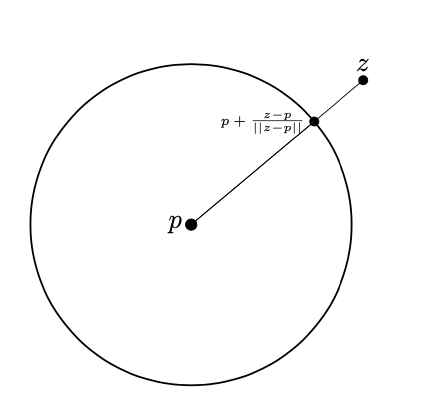
\includegraphics[scale = 0.5]{fotos_topo_2/otrasfotos/asdf.png}
    \end{equation}
\end{proof}

\begin{ter}
[Teorema de Bolzano en dimensió 2]\label{ter:bolzano2dmi}\index{Teorema de Bolzano en dimensió 2} Sigui $F:D^2\rightarrow \mathbb{R}^2$ una aplicació contínua, $f = F_{|S^1}$ i $p\in\mathbb{R}^2\setminus\{f(S^1)\}$. Si $\mu(f,p)\not=0$, aleshores $p\in F(D^2)$.
\end{ter}
\begin{proof}
Fixat $p\in\mathbb{R}^2\setminus\{f(S^1)\}$ tal que $\mu(f,p)\not=0$, considerem l'aplicació
\begin{equation}
    \notag
    \begin{array}{rl}
        H:S^1\times I & \longrightarrow \mathbb{R}^2 \\
        (z,t) & \longmapsto F(zt)
    \end{array}
\end{equation}
Tot suposant que $p\not\in F(D^2)$, buscarem arribar a una contradicció. Sota aquest supòsit, podem prendre $\mathbb{R}^2\setminus\{p\}$ com a espai d'arribada de $H$. Però, com que $H(z,1) = F(z) = f(z)$ i $H(z,0) = F(0)$, $\forall z\in S^1$, llavors tindrem que $f$ és homòtopa a l'aplicació constant $z\mapsto F(0)$ en $\mathbb{R}^2\setminus\{p\}$, d'on, per la proposició anterior, $\mu(f,p) = \mu(z\mapsto F(0),p) = 0$, que contradiu la hipòtesis del teorema. Concloem així que cal que el punt $p\in\mathbb{R}^2$ sigui la imatge d'algun punt de $D^2$ per $F$.
\end{proof}


\subsection{Conjunt de teoremes clàssics de topologia del pla}

Vist el teorema de Bolzano al pla, veurem ara algunes de les conseqüències d'aquest teorema, que reben el nom de conjunt de teoremes clàssics de topologia del pla.

\begin{ter}
[Teorema de Poincaré-Bohl]\label{ter:poincarebohl}\index{Teorema de Poincaré-Bohl} Siguin $f$ i $g$ dues corbes tancades planes i $p\in\mathbb{R}^2$ un punt que no pertany a la imatge de cap d'elles. Si $\forall z\in S^1$ el segment que uneix $f(z)$ amb $g(z)$, que denotarem per $\overline{f(z)g(z)}$, no passa per $p$, llavors $\mu(f,p) = \mu(g,p)$.
\end{ter}
\begin{proof}
Per la proposició prèvia al teorema de Bolzano (\ref{prop:bolzano2dim}), serà suficient provar que sota les hipòtesis del resultat $f$ i $g$ són homòtopes a $\mathbb{R}^2\setminus\{p\}$. I això és trivial, ja que, per hipòtesis
\begin{equation}
    \notag
    \begin{array}{rl}
        H:S^1\times I & \longrightarrow\mathbb{R}^2\setminus\{p\} \\
        (z,t) & \longmapsto tf(z)+(1-z)g(z)
    \end{array}
\end{equation}
que no fa més que descriure el segment que uneix $f(z)$ amb $g(z)$ per cada $z\in S^1$, està ben definida i és evident que defineix una homotopia entre $f$ i $g$ a $\mathbb{R}^2\setminus\{p\}$.
\end{proof}


\begin{ter}
[Teorema de Rouché, exercici 13]\label{ter:teoremaderouche}\label{exercici2.13}\index{Teorema de Rouché} Donades dues corbes tancades planes $f$ i $g$, si $\forall z\in S^1$ es compleix
\begin{equation}
    \notag
    d(f(z),g(z))\leq \max\{d(p,f(z)),d(p,g(z))\}
\end{equation}
llavors $\mu(f,p) = \mu(g,p)$.
\end{ter}
\begin{proof}
Usant el teorema anterior, serà suficient veure que, sota els supòsits donats, $p$ no pertany al segment $\overline{f(z)g(z)}$ per cap $z\in S^1$. I això es veu ràpidament per reducció a l'absurd: si $\exists z_*\in S^1$ tal que $p\in \overline{f(z_*)g(z_*)}$, llavors la distància de $p$ a $f(z_*)$ i $g(z_*)$ ha de ser menor que la distància de $f(z_*)$ a $g(z_*)$, que no és sinó la longitud del segment $\overline{f(z_*)g(z_*)}$. D'aquí es desprèn que $d(f(z_*),g(z_*))>\max\{d(p,f(z_*)),d(p,g(z_*))\}$, que contradiu les nostres hipòtesis.
\end{proof}

\begin{ej}
Veiem un exemple d'aquest teorema: Si $p$ és la posició del Sol (que suposem fix), $\alpha(t)$ la trajectòria de la Lluna i $\beta(t)$ la trajectòria de la Terra, com que la distància de la Terra i la Lluna és sempre menor que la de la Terra al Sol, el Teorema de Rouché anterior ens diu que el nombre de voltes al voltant del Sol que dona la Terra en un determinat període de temps, és el mateix que el de la Lluna. De fet, el pla de l'òrbita de la Lluna al voltant de la Terra està lleugerament inclinat respecte al pla d'òrbita de la Terra al voltant del Sol, l'anomenat pla d'eclíptica, i per tant aquest exemple no és del tot correcte. Per corregir aquesta incorrecció és usual prendre $\beta(t)$ com la projecció ortogonal sobre el pla de l'eclíptica de la trajectòria de la Lluna.
\end{ej}

\begin{ter}
[Teorema d'estabilitat]\label{ter:teoremaestabilitat}\index{Teorema d'estabilitat} Donada una corba tancada plana $f$ i un punt $p\in \mathbb{R}^2$ que no pertany a la seva imatge (és a dir, $p\not\in f(S^1)$), tenim:
\begin{enumerate}[(i)]
    \item Per un cert $\varepsilon>0$, per tota corba tancada plana $g$ tal que $\displaystyle\sup_{z\in S^1}\{d(f(z),g(z))\}<\varepsilon$ se satisfà $p\not\in g(S^1)$ i $\mu(f,p) = \mu(g,p)$.
    \item Si $q\in \mathbb{R}^2$ pertany a la component arc-connexa de $\mathbb{R}^2\setminus f(S^1)$ que conté $p$, llavors $\mu(f,p) = \mu(f,q)$.
    \begin{equation}
    \notag
    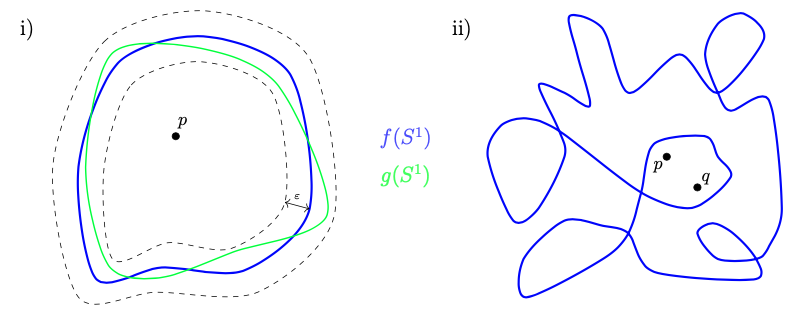
\includegraphics[scale = 0.8]{fotos_topo_2/otrasfotos/teoremaestabilitat.png}
    \end{equation}
\end{enumerate}
\end{ter}
\begin{proof}
\begin{enumerate}[(i)]
    \item Veurem que $\varepsilon = d(f(S^1),p)$ compleix les propietats que busquem. Notem primer que, essent $f$ una aplicació contínua i $S^1$ un conjunt compacte, $f(S^1)$ és també un conjunt compacte i, per ser-ho en $\mathbb{R}^2$, serà també tancat. Així doncs, com que, per hipòtesi, $p\not\in f(S^1)$, tindrem $\varepsilon>0$.

Ara, donada una corba $g$ tal que $\sup_{z\in S^1}\{d(f(z),g(z))\}<\varepsilon$, si $g(z_*) = p$ per un cert $z_*\in S^1$, llavors passaria
\begin{equation}
    \notag
    d(f(z_*),p) = d(f(z_*),g(z_*))\leq\sup_{z\in S^1}\{d(f(z),g(z))\}<\varepsilon =
\end{equation}
\begin{equation}
    \notag
    = d(p,f(S^1)) = \inf_{z\in S^1}\{d(p,f(z))\}\leq d(p,f(z_*))
\end{equation}
Concloem amb aquesta contradicció que $p\not\in g(S^1)$. Generalitzant aquesta cadena de desigualtats, $\forall z\in S^1$, tenim
\begin{equation}
    \notag
    d(f(z),g(z))<d(f(z),p)\leq \max\{d(f(z),p),d(g(z),p\}
\end{equation}
En altres paraules, $f$ i $g$ satisfan les hipòtesis del teorema de Rouché i, per tant, $\mu(f,p) = \mu(g,p)$.

\item Essent $p$ i $q$ d'una mateixa component arc-connexa, podem prendre un camí continu $\gamma:[0,1]\rightarrow \mathbb{R}^2\setminus S^1$ tal que $\gamma(0) = p$ i $\gamma(1) = q$. Com que, per construcció, aquest camí no talla la imatge de $f$, llavors l'aplicació
\begin{equation}
    \notag
    \begin{array}{rl}
        H:S^1\times I & \longrightarrow S^1 \\
        (z,t) & \longmapsto\frac{f(z)-\gamma(t)}{\|f(z)-\gamma(t)\|}
    \end{array}
\end{equation}
està ben definida i és contínua. De fet, $H$ és una homotopia entre $N_p\circ f$ i $N_q\circ g$, ja que satisfà 
\begin{equation}
    \notag
    H(z,0) = \frac{f(z)-\gamma(0)}{\|f(z)-\gamma(0)\|} = \frac{f(z)-p}{\|f(z)-p\|} = (N_p\circ f)(z)\;\forall z\in S^1 
\end{equation}
\begin{equation}
    \notag
    H(z,1) = \frac{f(z)-\gamma(1)}{\|f(z)-\gamma(1)\|} = \frac{f(z)-q}{\|f(z)-q\|}=(N_q\circ f)(z)\;\forall z\in S^1
\end{equation}
Amb tot, per la definició de l'índex i la invariància del grau per homotopies,
\begin{equation}
    \notag
    \mu(f,p) = \mathrm{gr}(N_p\circ f) = \mathrm{gr}(N_q\circ f) = \mu(f,q).
\end{equation}
\end{enumerate}
\end{proof}

\begin{ej}
Siguin $f:S^1\rightarrow \mathbb{C}\simeq\mathbb{R}^2$ la corba tancada plana definida com $f(z) = z^n,\;\forall z\in S^1$ per un cert $n\geq 1$ i considerem el punt $p\in \mathbb{C}\setminus f(S^1) = \mathbb{C}\setminus S^1$.

Si $\|p\|<1$, llavors $p$ pertany a la mateixa component arc-connexa que $0\in\mathbb{C}$, d'on valent-nos del segon apartat del teorema d'estabilitat (\ref{ter:teoremaestabilitat}), $\mu(f,p) = \mu(f,0)=\mathrm{gr}f = n$.

Per contra, si $\|p\|>1$, notem que si $g:S^1\rightarrow \mathbb{R}^2$ és l'aplicació constant igual a 0, llavors $p\not\in\overline{f(z)g(z)}$ $\forall z\in S^1$. Per tant, podem usar el teorema de Poincaré-Bohl (\ref{ter:poincarebohl}) per afirmar que $\mu(f,p) = \mu(g,p) = 0$.
\end{ej}


\begin{ter}
[Teorema fonamental de l'àlgebra]\label{ter:teoremafonamentaldelalgebra}\index{Teorema fonamental de l'àlgebra} Per tot polinomi $p(z)\in\mathbb{C}[z]$ existeix $\alpha\in \mathbb{C}$ tal que $p(\alpha)=0$.
\end{ter}
\begin{proof}
Escrivim el polinomi $p(z) = z^n+a_{n-1}z^{n-1}+\cdots +a_1z+a_0$ on $n\geq 1$ i $a_i\in\mathbb{C}$, $\forall i=1,\ldots, n-1\}$. Considerem $\lambda = 1+\|a_{n-1}\|+\cdots+\|a_1\|+\|a_0\|>1$. Si $\lambda= 1$, aleshores $p(z) = z^n$ i per tant, $\alpha = 0$ és una arrel de $p$. Suposem que $\lambda>1$ i prenem les aplicacions
\begin{equation}
    \notag
    \begin{array}{rl}
        F:D^2 & \longrightarrow \mathbb{C} \\
        z & \longmapsto p(\lambda z)
    \end{array}
    \qquad
    \begin{array}{rl}
        \sigma:S^1 & \longrightarrow \mathbb{C} \\
        z & \longmapsto (\lambda z)^n
    \end{array}
\end{equation}
i $f = F_{|S^1}$. Observem que $\sigma$ retorna per cada $z\in S^1$ el coeficient líder de $f$. Serà suficient provar que $\mu(f,0)\not=0$, ja que en tal cas, pel teorema de Bolzano, $\exists z_0\in D^2$ tal que $F(z_0) = 0$, i.e. $\lambda z_0$ és una arrel de $p$., Per veure que se satisfà aquesta propietat, usarem el teorema de Rouché per comparar l'índex de $f$ respecte 0 amb el de $\sigma$. Concretament, tenim que si $z\in  S^1$, llavors
\begin{equation}
    \notag
    d(f(z),\sigma(z)) = \|f(z)-\sigma(z)\| = \|a_{n-1}(\lambda z)^{n-1}+\cdots+a_1\lambda z+a_0\|\leq
\end{equation}
\begin{equation}
    \notag
    \leq \|a_{n-1}\lambda^{n-1}z^{n-1}\|+\cdots+\|a_1\lambda z\|+\|a_0\| = \|a_{n-1}\lambda^{n-1}\|+\cdots+\|a_1\lambda\|+\|a_0\|\leq 
\end{equation}
\begin{equation}
    \notag
    \leq \lambda^{n-1}(\|a_{n-1}\|+\cdots+\|a_1\|+\|a_0\|) \leq \lambda^n = \|\sigma(z)-0\|
\end{equation}
En definitiva, $d(f(z),\sigma(z))\leq d(\sigma(z),0)\leq\max\{d(\sigma(z),0),d(f(z),0)\}$, d'on, per Rouché, $\mu(f,0) = \mu(\sigma,0) = \mathrm{gr}(z\mapsto z^n) = n\leq 1>0$.
\end{proof}


\begin{ter}
[Teorema de Borsuk-Ulam]\label{ter:teoremadeborsukulam}\index{Teorema de Borsuk-Ulam} Tota aplicació contínua $f:S^2\rightarrow\mathbb{R}^2$ amb la propietat $f(z)= -f(-z)$ $\forall z\in S^2$ s'anul·la en un cert $p_0\in S^2$, és a dir, $\exists p_0\in S^2$ tal que $f(p_0) = (0,0)$.
\end{ter}
\begin{proof}
Sigui $F = \pi^{-1}\circ f$, on $\pi$ denota la projecció de $S^2$ sobre el disc unitat del pla, de manera que $F$ és l'aplicació
\begin{equation}
    \notag
    \begin{array}{rl}
        F:D^2 & \longrightarrow\mathbb{R}^2 \\
        (x,y) & \longmapsto \left(x,y,\sqrt{1-(x^2+y^2)}\right)
    \end{array}
\end{equation}
Serà suficient veure que $(0,0)\in F(D^2)$. Concretament, veurem que si $(0,0)\not\in F(S^1)$, llavors $F$ s'anul·la per algun punt de l'interior del disc $D^2$. Notem per això que $F$ és contínua i, si $(x,y)\in S^1$, és a dir, $x^2+y^2=1$, satisfà
\begin{equation}
    \notag
    F(x,y) = f(x,y,0) = -f(-x,-y,0) = -F(-x,-y)
\end{equation}
Havent suposat que l'origen no és la imatge de $S^1$ per $F$, podem calcular l'índex d'aquesta funció restringida a la circumferència respecte $(0,0)\in D^2$. Per fer-ho, prenem $g = N_0\circ F_{|S^1}$ i una elevació $\tilde{g}$ del camí $g\circ e$. Així, com que, amb el que hem vist abans, $g(-z) = -g(z)\;\forall z\in S^1$ i, per la definició d'elevació (\ref{def:elevaciodecamins}), $g(z)=e^{2\pi i\tilde{g}(t)}\;\forall z = e^{2\pi it}\in S^1$, en particular si $t\in [0,1/2]$,
\begin{equation}
    \notag
    e^{2\pi i\tilde{g}(t)} = g(z) = -g(-z) = e^{\pi i}g(e^{\pi i}e^{2\pi it} = e^{\pi i}g(e^{2\pi i(t+1/2)}) = e^{\pi i}e^{2\pi i\tilde{g}(t+1/2)} \Longrightarrow
\end{equation}
\begin{equation}
    \notag
    \Longrightarrow k(t) = \tilde{g}(t)-\frac{1}{2}-\tilde{g}(t+\frac{1}{2})\in\mathbb{Z}.
\end{equation}
Com $\tilde{g}$ és contínua, $k$ també ho serà i, de fet, com que $I$ és connex, $k$ és constant, sigui $k_0\in\mathbb{Z}$ el valor que pren $k(t)$ per $t\in [0,1/2]$. Llavors,
\begin{equation}
    \notag
    \left.
    \begin{array}{ll}
        k_0 = k(0) = \tilde{g}(0)-\frac{1}{2}-\tilde{g}(\frac{1}{2})\\
        k_0 = k(\frac{1}{2}) = \tilde{g}(\frac{1}{2})-\frac{1}{2}-\tilde{g}(1)
    \end{array}
    \right\} \Rightarrow 2k_0=\tilde{g}(0)-\tilde{g}(1) -1
\end{equation}
d'on $\mu(F_{|S^1},(0,0))=\mathrm{gr}g = \mathrm{gr}(g\circ e) = \tilde{g}(1)-\tilde{g}(0) = -2k_0-1\not=0$ atès que $k_0$ és un enter. I d'aquí, pel Teorema de Bolzano (\ref{ter:bolzano2dmi}), $(0,0)\in F(D^2)$.
\end{proof}

\begin{coro}[Variant del teorema de Borsuk-Ulam]
Aquest teorema és equivalent al fet que tota aplicació contínua de l'esfera al pla admet un punt $p_1\in S^2$ la imatge del qual coincideix amb la del seu punt antipodal, i.e. $\forall g:S^2\rightarrow \mathbb{R}^2$ contínua $\exists p_1\in S^2$ tal que $g(p_1) = g(-p_1)$
\end{coro}
\begin{proof}
Comencem per observar que donada una certa $g:S^2\longrightarrow\mathbb{R}^2$ contínua, l'aplicació $f(z) = g(z)-g(-z)$ és també contínua i satisfà
\begin{equation}
    \notag
    -f(-z) = -(g(-z)-g(-(-z))) = g(z)-g(-z) = f(z)\;\;\;\forall z\in S^2
\end{equation}
Així, si el teorema (\ref{ter:teoremadeborsukulam}) és cert, podem trobar $p_0\in S^2$ pel qual $f(p_0) = g(p_0)-g(-p_0) = 0$, de manera que el punt complexi $g(p_0)=g(-p_0)$.
\end{proof}

\begin{ter}
[Teorema de Lusternik-Schirelmann]\label{ter:lusternikschirelmann}\index{Teorema de Lusternik-Schirelmann} Donats tres conjunts tancats qualssevol $A,B,C\subset S^2$ tals que $A\cup B\cup C = S^2$, almenys un d'ells conté una parella de punts antípodes.
\end{ter}
\begin{proof}
Sigui $g:S^2\rightarrow \mathbb{R}^2$ definida com $g(p) = (d(p,A),d(p,g))$, $\forall p\in S^2$. Aquesta funció és clarament contínua i, per tant, per la variant del teorema de Borsuk-Ulam vista abans, $\exists p_1\in S^2$ tal que $g(p_1)=g(-p_1)$. Sigui $(\alpha,\beta)\in\mathbb{R}^2$ la imatge de $p_1$ per $g$. Si $\alpha = 0$ llavors $d(p_1,A) = d(-p_1,A)=0$; equivalentment, essent $A$ tancat, cal $p_1,-p_1\in\overline{A}=A$. Anàlogament, si $\beta = 0$, aleshores $p_1,-p_1\in B$. Finalment, si $\alpha,\beta\not=0$, tindrem $p_1,-p_1\not\in A\cup B$,, d'on, com que $p_1,-p_1\in S^2=A\cup B\cup C$, necessàriament $p_1,-p_1\in C$.
\end{proof}


\subsection{El tipus d'homotopia d'un graf}

\begin{defi}
[Graf]\label{def:graf}\index{Graf} Un \textit{graf finit (geomètric)} és un espai topològic $G$ amb una família finita de punts de $G$, $\{v_i\}_{i\in V}$, anomenats els \textit{vèrtexs} de $G$, i una família finita de compactes de $G$, $\{a_j\}_{j\in E}$, anomenats les \textit{arestes} de $G$, tals que
\begin{itemize}
    \item $G$ és la reunió de totes les seves arestes
    \item Cada aresta onté un o dos vèrtexs, anomenats els \textit{vèrtexs de l'aresta}
    \item El complementari en cada aresta dels seus vèrtexs és homeomorf a l'interval $(0,1)$
    \item Dues arestes no disjuntes s'intersequen només en vèrtexs.
\end{itemize}
\end{defi}

\begin{ter}
\label{ter:numerodebetti} Sigui $G$ un graf connex amb $v$ vèrtexs i $a$ arestes. Aleshores $G$ és homotòpicament equivalent a la unió puntual de $\ell$ circumferències, essent $\ell = 1-v+a$ i, per tant, $\pi(G)\cong \mathbb{F}_\ell$. A $\ell$ se li diu \textit{nombre de llaços}\index{Nombre de llaços}\index{Primer nombre de Betti} (o primer nombre de Betti) de $G$.
\end{ter}
\begin{proof}
Per inducció sobre el nombre $v$ de vèrtexs. 

Si $v = 1$, aleshores $G$ ja és la unió puntual d'$a$ circumferències i per tant $\pi(G)\cong \mathbb{F}_a$ que prova el teorema en aquest cas.

Suposem el resultat cert per a $v-1$ vèrtex i suposem que ara $G$ té $v$ vèrtexs. Aleshores existirà una aresta amb vèrtexs diferents, ja que $G$ és connex. Contraient aquesta aresta a un punt, s'obté un nou graf $G'$ amb $v'$ vèrtexs i $a'$ arestes, tal que $v' = v-1$ i $a' = a-1$. Per hipòtesis d'inducció, $G'$ serà homotòpicament equivalent a la unió puntual de $\ell'$ circumferències, on $\ell' = 1-v'+a'$. Però com que $\ell' = 1-v'+a'=1-(v-1)+(a-1)=1-v+a=\ell$ i $G'$ és del mateix tipus d'homotopia que $G$, resulta que $G$ és homotòpicament equivalent a la unió puntual de $\ell$ circumferències i per tant $\pi(G)\cong \mathbb{F}_\ell$.
\end{proof}
\begin{defi}
[València o grau d'un vèrtex]\label{def:valencia}\index{València d'un vèrtex}\index{Grau d'un vèrtex} Si $v$ és un vèrtex del graf $G$, s'anomena \textit{valència} o bé \textit{grau de $v$}, a $d(v) = \#\{a\;:\;a$ aresta de $G$ amb dos vèrtexs diferents$\}+2\#\{a\;:\;a$ aresta de $G$ amb $v$ com a únic vèrtex$\}$. Un graf que té tots els seus vèrtexs amb grau $d = 3$ s'anomena \textit{trivalent}\index{Graf trivalent}\label{def:graftrivalent}.
\end{defi}








\subsection{Exercicis proposats}
\begin{exercici}
[Exercici 4]\label{exercici2.4} Considerem el grup ortogonal especial $SO(3)$, format per les matrius de les rotacions a $\mathbb{R}^3$, amb la topologia euclidiana i punt base la matriu identitat.
\begin{enumerate}[(a)]
    \item Demostreu que $SO(3)$ és homeomorf a $\mathbb{R}P^3$.
    \item Demostreu que si $\rho$ denota el llaç a $SO(3)$ definit per les rotacions al voltant de l'eix $x = y = 0$, llavors $\rho*\rho$ és homòtop al llaç constant en el punt base.
\end{enumerate}
\end{exercici}
\begin{sol}
Recordem que el grup aquest és
\begin{equation}
    \notag
    X = SO(3,\mathbb{R}) = \left\{A\in M(3,3,\mathbb{R})\;:\;AA^t=\mathrm{Id},\;\det A=1\right\}\subseteq\mathbb{R}^9
\end{equation}
\begin{enumerate}[(a)]
    \item No lo sé
    \item $[\rho]\in\pi(X,\mathrm{Id})$, on $\rho$ és un llaç de rotacions\footnote{Ho podem pensar com si fóssim cambrers que portem una safata plena de copes de vidre subjectada amb una mà. Aleshores la fem girar sense que es caigui res i que no se'ns retorci el braç. Aleshores el que fem és un camí tancat. En física s'anomena ``spin''. Les partícules \textit{spin} són les que responen a la $\rho$.} al voltant de l'eix $x=y=0$. 
    
    Representem amb matrius:
    \begin{equation}
        \notag
        \rho(s) = \begin{pmatrix}
        \cos 2\pi s & -\sin 2\pi s & 0 \\
        \sin 2\pi s & \cos 2\pi s & 0 \\
        0 & 0 & 1
        \end{pmatrix}
        \qquad 0\leq s\leq 1
    \end{equation}
    \begin{equation}
        \notag
        \overline{\rho}(s) = \rho(1-s)= \begin{pmatrix}
        \cos 2\pi s & \sin 2\pi s & 0 \\
        -\sin 2\pi s & \cos 2\pi s & 0 \\
        0 & 0 & 1
        \end{pmatrix}
    \end{equation}
    Aleshores, el problema és demostrar que $\rho^2\simeq \varepsilon_{\mathrm{Id}}$ (camí constant en Id). Això és equivalent a demostrar que $\rho\simeq \overline{\rho}$. Definim doncs
    \begin{equation}
        \notag
        H(s,t) = \begin{pmatrix}
        1 & 0 & 0 \\
        0 & \cos\pi t & \sin\pi t \\
        0 & -\sin\pi t & \cos \pi t
        \end{pmatrix} \rho \begin{pmatrix}
        1 & 0 & 0 \\
        0 & \cos\pi t & -\sin\pi t \\
        0 & \sin\pi t & \cos \pi t
        \end{pmatrix}
    \end{equation}
    Aquesta és una homotopia ja que és una matriu ortogonal de determinant 1 (per tant és de $SO(3,\mathbb{R})$ contínua i es pot comprovar que satisfà totes les condicions d'homotopia.
\end{enumerate}
\end{sol}




\begin{exercici}
[Exercici 7]\label{exercici2.7} Demostreu que, si $D^2$ denota el disc unitat tancat de $\mathbb{R}^2$ i $f:D^2\rightarrow D^2$ és un homeomorfisme, llavors $f(S^1)=S^1$.
\end{exercici}
\begin{sol}
Veiem en primer lloc la inclusió $f(S^1)\subseteq S^1$. Si no fos així, existiria algun $x\in S^1$ tal que $y=f(x)\in (D^2)^\circ = D^2\setminus S^1$. Però com $f$ és un homeomorfisme, també ho és $f_{|D^2\setminus\{x\}}$ i per tant $D^2\setminus\{x\}\simeq D^2\setminus\{y\}$ que implica que $\pi(D^2\setminus\{x\})\cong \pi(D^2\setminus\{y\})$ (per \ref{ter:invarianciatopologicadelgrupfonamental}). Ara bé, $D^2\setminus\{x\}$ és convex, i per tant $D^2\setminus\{x\}\simeq *$, i així $\pi(D^2\setminus\{x\}) = 0$ (on 0 denota el grup trivial). Mentre que $D^2\setminus\{y\}\simeq S^1$ (per l'exercici ?? de la llista 1) i per tant $\pi(D^2\setminus\{y\})\cong \mathbb{Z}$ pel que ja hem vist. Per tant contradiu l'isomorfisme $\pi(D^2\setminus\{x\})\cong \pi(D^2\setminus\{y\})$ i arribem a una contradicció. Per tant ha de ser $f(S^1)\subseteq S^1$.

Per fer la inclusió contraria, només cal aplicar el mateix raonament a $g = f^{-1}$ i aleshores es pot concloure que $f^{-1}(S^1)\subseteq S^1$ cos que implica que $S^1\subseteq f(S^1)$ i juntament amb la inclusió anterior obtenim la igualtat.
\end{sol}



\begin{exercici}
[Exercici 8]\label{exercici2.8} Demostreu que tota aplicació contínua $S^2\rightarrow S^2$ no exhaustiva té algun punt fix.
\end{exercici}
\begin{sol}
Sigui $f:S^2\rightarrow S^2$ una aplicació contínua no exhaustiva. Com $f$ no és exhaustiva, existeix un punt $p\in S^2\setminus \mathrm{Im}f$. Equivalentment $\mathrm{Im}f\subseteq S^2\setminus\{p\}$. Ara bé, $S^2\setminus\{p\}\simeq \mathbb{R}^2$ (per la projecció estereogràfica) i com $\mathrm{Im}f$ és compacte, existeix un compacte $K\simeq D^2$ tal que $\mathrm{Im}f\subseteq K\subseteq S^2\setminus\{p\}$.

Considero la restricció de $f$ al compacte $K$, és a dir, $f_{|K}=g:K\rightarrow K$. Com $K\simeq D^2$ i $D^2$ satisfà la PPF pel Teorema de Brouwer (\ref{ter:puntfixbrouwer}), per (\ref{exercici2.11.b}) $K$ satisfà la PPF i per tant $g$ té un punt fix (és a dir, $\exists z_0\in K$ tq $g(z_0) = z_0$). En definitiva, com $g=f_{|K}$, es té que $f$ té un punt fix.
\end{sol}


\begin{exercici}
[Exercici 9]\label{exercici2.9} Sigui $X = \{(x,y)\in\mathbb{R}^2\;:\;1\leq x^2+y^2\leq 4\}$. Demostreu que tota aplicació contínua $X\rightarrow X$ homòtopa a una aplicació constant té algun punt fix.
\end{exercici}
\begin{sol}
Considerem la corona $X$ donada a l'enunciat. Sigui $H:X\times I\rightarrow X$ l'homotopia tal que $H(x,1) = f(x)$, $H(x,0) = \varepsilon_{x_0}(x) = x_0\in X$, $\forall x\in X$, és a dir, la homotopia que dona la equivalència $f\simeq \varepsilon_{x_0}$, on $\varepsilon_{x_0}$ és l'aplicació constant que sempre dona $x_0$.

Sigui $D^2_2(0) = \{(x,y)\in\mathbb{R}^2\;:\;x^2+y^2\leq 4\}$ el disc tancat de radi 2 i centre 0, i definim l'aplicació
\begin{equation}
    \notag
    g:D_2^2(0)\longrightarrow X\subseteq D_2^2(0)
\end{equation}
per $g(x,y) = f(x,y)$, si $(x,y)\in X$; $g(x,y) = H\left(\frac{(x,y)}{\|(x,y)\|},\|(x,y)\|\right)$, si $0<x^2+y^2\leq 1$ i $g(0,0)=x_0$. Aquesta aplicació està ben definida ja que, si $x^2+y^2=1$, $H((x,y),1)= f(x,y)$ i és contínua ja que ho és $H$.

Ara, pel Teorema del Punt Fix de Brouwer (\ref{ter:puntfixbrouwer}) $g$ té un punt fix, és a dir, existeix $x_0$ tal que $g(x_0) = x_0$. Com $\mathrm{Im}g\subseteq X$, $x_0\in X$. Finalment, donat que sobre $X$, $g=f$, concloem que $f(x_0) = g(x_0) = x_0$ i per tant $f$ té un punt fix.
\end{sol}


\begin{exercici}
[Exercici 10]\label{exercici2.10} Demostreu que tota matriu $3\times 3$ amb coeficients positius té algun valor propi positiu.
\end{exercici}
\begin{sol}
Notem $K$ l'octant positiu de $S^2$ (és a dir, $K = \{(x,y,z)\in\mathbb{R}^3\;:\;x\geq 0,\;y\geq 0,\;z\geq 0\}\cap S^2$). Aquest octant és homotòpicament equivalent al disc tancat $D^2$. Notem $A$ una matriu amb tots els elements positius. Podem considerar l'aplicació
\begin{equation}
    \notag
    \begin{array}{rl}
        f:K & \longrightarrow K \\
        x & \longmapsto \frac{A(x)}{\|A(x)\|}
    \end{array}
\end{equation}
Aquesta aplicació no estarà ben definida si existeix algun $x_0$ tal que $A(x_0)=0$, però si passa això, $A$ té el valor propi $\lambda = 0$. Aleshores, podem suposar que $A(x)\not=0$ per qualsevol $x$ i així $f$ està ben definida amb aquesta hipòtesi.

Com $f$ és contínua, pel Teorema del Punt Fix de Brouwer (\ref{ter:puntfixbrouwer}) i per (\ref{exercici2.11.b}), existeix un $x_0$ tal que $f(x_0) = x_0$, és a dir, $\frac{A(x_0)}{\|A(x_0)\|}=x_0$, $x_0\in S^2$. O sigui, $A(x_0)=\|A(x_0)\|x_0$, $x_0\in S^2$. Per tant, $A$ té el VAP $\|A(x_0)\|>0$.
\end{sol}



\begin{exercici}
[Exercici 14]\label{exercici2.14} Calculeu l'índex del camí tancat
\begin{equation}
    \notag
    \gamma(t) = e^{4\pi it}+e^{2\pi it}+1,\qquad 0\leq t\leq 1
\end{equation}
al pla complex respecte als punts $p_1=0.5$, $p_2 = 4$, $p_3=1+i$.
\end{exercici}
\begin{sol}
Primer cal destacar que grau d'un camí (\ref{def:graudecami}) és el mateix que índex d'un camí. Així doncs, el que volem calcular és el grau del camí $\gamma(t) = e^{4\pi it}+e^{2\pi it}+1$. Podem expressar aquest camí com la composició
\begin{equation}
    \notag
    \begin{array}{rll}
        I & \longrightarrow S^1 & \overset{\alpha}{\longrightarrow} \mathbb{C} \\
        t & \longmapsto e^{2\pi it} & \longmapsto e^{4\pi it}+e^{2\pi it}+1
    \end{array}
\end{equation}
essent $\alpha(z) = z^2+z+1$.

Podríem considerar, més en general, que $\alpha(z)$ fos un polinomi en $z$ qualsevol, ja que el mètode de la solució d'aquest exercici seria anàleg, i es basa en les propietats de l'índex de (\ref{prop:propietatsindex}). Tenint en compte aquestes propietats, doncs, resoldrem l'exercici calculant l'índex de $\alpha$, ja que $\gamma = \alpha\circ e$, on $e$ és la funció exponencial. Així doncs, calculem-lo en cada cas:
\begin{itemize}
    \item \underline{$p_1 = \frac{1}{2}$} $\mu(z^2+z+1,1/2) = \mu(z^2+z+1-1/2,0) = \mu(z^2+z+1/2,0)$. Ara trobem les arrels de $z^2+z+\frac{1}{2} = 0$, que són $z = \frac{-1\pm i}{2}$, i per tant,
    \begin{equation}
        \notag
        \mu(z^2+z+1/2,0) = \mu\left(z-\frac{-1+i}{2},0\right)+\mu\left(z-\frac{-1-i}{2},0\right) = 
    \end{equation}
    \begin{equation}
        \notag
        =\mathrm{gr}\frac{\alpha}{\|\alpha\|}+\mathrm{gr}\frac{\beta}{\|\beta\|}=\mu(\alpha,0)+\mu(\beta,0).
    \end{equation}
    Ara veiem que les dos arrels tenen mòdul $\left\|\frac{-1\pm i}{2}\right\|=\frac{\sqrt{2}}{2}<1$ i aleshores resulta que $(*)=1+1=2$.
    \item \underline{$p_2 = 4$}. Procedim d'una manera similar:
    \begin{equation}
        \notag
        \mu(z^2+z+1,4)=\mu(z^2+z+1-3,0) = \mu\left(z,\frac{-1+\sqrt{13}}{2}\right)+\mu\left(z,\frac{-1-\sqrt{13}}{2}\right) = 0
    \end{equation}
    ja que $\left\|\frac{-1\pm\sqrt{13}}{2}\right\|>1$.
    \item \underline{$p_3 = 1+i$}. En aquest cas tenim
    \begin{equation}
        \notag
        \mu(z^2+z+1,1+i) = \mu(z^2+z-i,0) = (*)
    \end{equation}
    les arrels de $z^2+z-i=0$ són $z_{\pm}\frac{1}{2}(-1\pm\sqrt{1+4i})$ que tenen mòdul $\|z_+\|>1$ i $\|z_-\|<1$ i per tant $(*) = 0+1=1$.
\end{itemize}
\end{sol}





\begin{exercici}
[Exercici 16]\label{exercici2.16} \begin{enumerate}[(a)]
    \item Demostreu que, si una aplicació contínua $g:S^1\rightarrow S^1$ es pot estendre a una aplicació contínua $D^2\rightarrow S^1$, on $D^2$ denota el disc tancat, llavors $g$ té grau 0.
    \item Siguin $f$ i $g$ dues aplicacions contínues $D^2\rightarrow D^2$. Demostreu que $g(S^1)\subset S^1$ i el grau de la restricció $g:S^1\rightarrow S^1$ és diferent de zero, llavors hi ha algun punt $x_0\in D^2$ tal que $f(x_0) = g(x_0)$.
    \item Calculeu el grau de l'aplicació $g:S^1\rightarrow S^1$ donada per $g(x,y) = (x^2-y^2,2xy)$.
    \item Demostreu que el sistema d'equacions següent té alguna solució a $\mathbb{R}^2$:
    \begin{equation}
        \notag
        \left\{
        \begin{array}{ll}
            \cos(x+y+y^2)-x^2+y^2 = 0 \\
            \sin(x+y+y^2)-2xy=0.
        \end{array}
        \right.
    \end{equation}
\end{enumerate}
\end{exercici}
\begin{sol}
\begin{enumerate}[(a)]
    \item Si $g:S^1\rightarrow S^1$ s'estén a una aplicació $G:D^2\rightarrow S^1$, vol dir que, notant $i:S^1\rightarrow D^2$ la inclusió, es té
    \begin{equation}
        \notag
        g = G\circ i:S^1\overset{i}{\longrightarrow}D^2\overset{G}{\longrightarrow}S^1
    \end{equation}
    Per tant, al passar a grups fonamentals tenim
    \begin{equation}
        \notag
        g_* = G_*\circ i_*:\pi(S^1)\rightarrow \pi(D^2)\rightarrow\pi (S^1)
    \end{equation}
    on hem demostrat ja que $\pi(S^1)\cong \mathbb{Z}$ i $\pi(D^2)\cong \{0\}$ (grup trivial). Per tant, resulta que 
    \begin{equation}
        \notag
        \mathrm{gr}g = g_*(1)=G_*(i_*(1))=G_*(0)=0.
    \end{equation}
    \item Com a la demostració del TPFB (\ref{ter:puntfixbrouwer}), si $f(x)\not=g(x)$, $\forall x\in D^2$, podem prendre la recta que passa per aquests dos punts $f(x)$ i $g(x)$ i després prendre el punt d'intersecció d'aquesta recta amb $S^1$, prenent el que estigui més a prop de $g(x)$. Així definim una aplicació contínua $r:D^2\rightarrow S^1$ que estén $g_{|S^1}$ ja que si $x\in S^1$, $g(x)$ ja pertany a $S^1$ i per tant $g(x)=r(x)$, $\forall x\in S^1$.
    
    Obtenim així que $g_{|S^1}$ s'estén a $D^2$ i per l'apartat (a), deurà ser $\mathrm{gr}g_{|S^1}=0$. Però la hipòtesis és que $\mathrm{gr}g_{|S^1}\not=0$, contradicció.
    \item L'aplicació $g(x,y) = (x^2-y^2,2xy)$ escrita utilitzant els complexos $z = x+iy\in\mathbb{C}$, és $g(z) = z^2$, i per tant $\mathrm{gr}(g)=2$. En general, $\mathrm{gr}(z^n) = n$.
    
    \item El sistema d'equacions donat es pot interpretar com l'equació $f(z) = g(z)$, on $f(x,y) = (\cos(x+y+y^2),\sin(x+y+y^2))$ i $g(x,y) = (x^2-y^2,2xy)$, suposant $z=x+iy\in\mathbb{C}$. Com que $\|f(z)\|,\|g(z)\|\leq 1$, $\forall z\in D^2$, i per l'apartat (c) $\mathrm{gr}(g_{|S^1})=2\not=0$ se satisfan les hipòtesis de l'apartat (b) i podem concloure que efectivament existeix un punt $(x_0,y_0)\in D^2$ tal que se satisfan les equacions.
\end{enumerate}
\end{sol}



\begin{exercici}
[Exercici 18]\label{exercici2.18} 
\begin{enumerate}[(a)]
    \item Demostreu que el camí tancat
    \begin{equation}
        \notag
        \gamma(t) = (5\cos 4\pi t + \sin^42\pi t-1,5\sin 4\pi t+\cos^72\pi t-2)
    \end{equation}
    no passa per $(0,0)$ i calcula l'índex de $\gamma$ respecte a $(0,0)$.
    \item Demostreu que el sistema d'equacions següent té alguna solució a $\mathbb{R}^2$ de mòdul menor que $0.70464$:
    \begin{equation}
        \left\{
        \begin{array}{ll}
            5x^2-5y^2+y^4=1 \\
            x^7+10xy = 2
        \end{array}
        \right.
    \end{equation}
    \item Comproveu que $x = 0.56548$, $y=0.35040$ és una solució.
\end{enumerate}
\end{exercici}
\begin{sol}
\begin{enumerate}[(a)]
    \item Considerem el camí 
    \begin{equation}
        \notag
        \begin{array}{rl}
            \alpha:I & \longrightarrow\mathbb{R}^2 \\
            t & \longmapsto (5\cos 4\pi t,5\sin 4\pi t) = 5e^{4\pi it}
        \end{array}
    \end{equation}
    que no passa per $(0,0)$ i té $\mu(\alpha,0)=2$. Com que per tot $t$,
    \begin{equation}
        \notag
        \|\gamma(t) = \alpha(t)\|= \sqrt{(\sin^4 2\pi t-1)^2+(\cos^72\pi t-2)^2}\leq
    \end{equation}
    \begin{equation}
        \notag
        \leq \sqrt{1+9}=\sqrt{10}<5 = \|\alpha(t)-(0,0)\|
    \end{equation}
    pel Teorema de Rouché (\ref{ter:teoremaderouche}) tenim que $\gamma$ no passa per 0 i $\mu(\gamma,0) = \mu(\alpha,0)=2$.
    
    \item Notem $D_r$ del disc de centre 0 i radi $r$ de $\mathbb{R}^2$, i $S_r$ la seva vora, és a dir, la circumferència de radi $r$. Considerem l'aplicació
    \begin{equation}
        \notag
        \begin{array}{rl}
            F:D_r & \longrightarrow \mathbb{R}^2 \\
            (x,y) & \longmapsto (5x^2-5y^2+y^4-1,x^7+10xy-2)
        \end{array}
    \end{equation}
    Si veiem que, per un cert $r>0$, $0\not\in F(S_r)$ i $\mu(F_{|S_r},0)\not=0$, tindrem, pel Teorema de Bolzano en dimensió 2 (\ref{ter:bolzano2dmi}) que $0\in F(D_r^\circ)$, és a dir, que el sistema té una solució de mòdul menor que $r$.
    
    Pel primer apartat, tenim que prenent $r=1$, els sistema té una solució de mòdul menor que 1. Ara, provar que si $r = 0.7\ldots$ es compleix també que $\mu(F_{|S_r},0)=2$ és refer l'apartat (a) amb aquesta $r$ concreta, cosa que no tornaré a fer.
\end{enumerate}
\end{sol}
    
    
    

\begin{exercici}
[Exercici 19]\label{exercici2.19} Per a cada regió delimitada per cadascun dels camins següents, determineu el nombre de voltes del camí respecte a un punt arbitrari situat a l'interior de la regió.
\begin{equation}
    \notag
    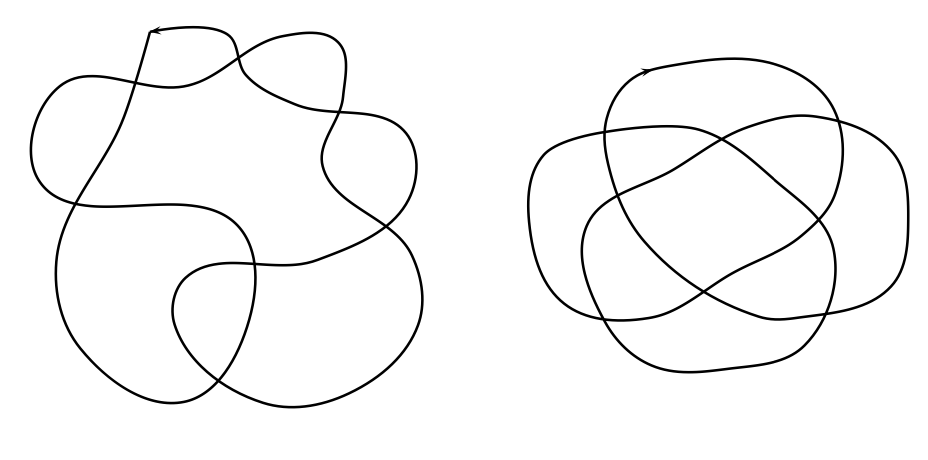
\includegraphics[scale = 0.5]{fotos_topo_2/otrasfotos/ex19.png}
\end{equation}
\end{exercici}
\begin{sol}
L'índex d'una corba amb respecte un punt de3pèn de la component connexa de $\mathbb{R}^2\setminus\alpha(I)$ en la que està el punt. És a dir, si $p$ i $q$ estan en la mateixa component de $\mathbb{R}^2\setminus\alpha(I)$ es té que $\mu(\alpha,p) = \mu(\alpha,q)$.

En efecte, podem prendre un camí $\gamma(s)$ tal que $\gamma(0) = p$ i $\gamma(1) = q$, i $\gamma(I) \subseteq\mathbb{R}^2\setminus\alpha(I)$. Aquest camí $\gamma$ ens permet definir l'homotopia
\begin{equation}
    \notag
    \begin{array}{rl}
        H:I\times I & \longrightarrow \mathbb{R}^2\setminus\{0\} \\
        (s,t) & \longmapsto H(s,t) = \dfrac{\alpha(t)-\gamma(s)}{\|\alpha(t)-\gamma(s)\|}
    \end{array}
\end{equation}
tal que $H(0,t) = \frac{\alpha(t)-p}{\|\alpha(t)-p\|}$, i $H(1,t) = \frac{\alpha(t)-q}{\|\alpha(t)-q\|}$, i per tant $\mu(\alpha,p) = \mathrm{gr}\frac{\alpha(t)-p}{\|\alpha(t)-p\|} = \mathrm{gr}\frac{\alpha(t)-q}{\|\alpha(t)-q\|} = \mu(\alpha,q)$.

Aleshores, utilitzant això, podem determinar:
\begin{equation}
    \notag
    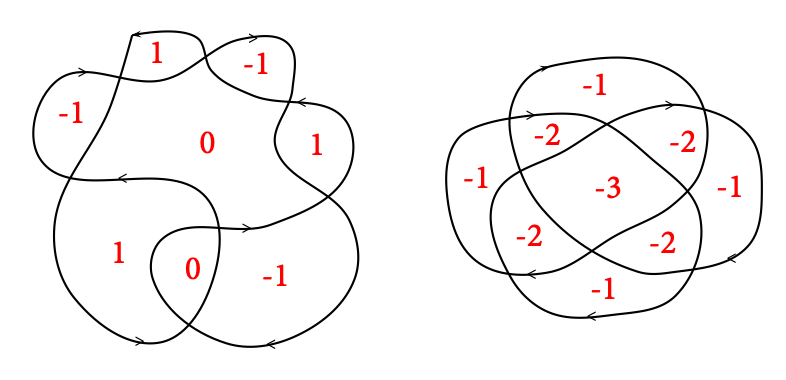
\includegraphics[scale = 0.5]{fotos_topo_2/otrasfotos/ex19sol.png}
\end{equation}
Bàsicament es tracta de comptar quantes voltes dona la corba dibuixada al voltant del punt que s'estudia. Si la volta és antihorari se li suma 1, si és horària se li resta 1.
\end{sol}









\section{El teorema de Seifert-Van Kampen}
\subsection{Grups lliures i presentacions de grups}

\begin{defi}
[Grup lliure]\label{def:gruplliure}\index{Grup lliure} Donat un conjunt $A = \{a_i\}_{i\in J}$ qualsevol, el \textit{grup lliure} generat per $A$ és el grup format per les \textit{paraules} (de llargària finita) $a_{i_1}^{m_1}a_{i_2}^{m_2}\cdots a_{i_r}^{m_r}$, on cada $a_{i_k}$ pertany a $A$ i cada exponent $m_k$ és un nombre enter. L'operació és la juxtaposició de paraules, amb les regles $a^ma^n = a^{m+n}$ i $a^0=1$ per a tot $a\in A$, on 1 és un símbol addicional que actua com a element neutre. Aquest grup es denota per $F(A)$\index{$F(A)$}.
\end{defi}

\begin{nota}
De vegades es troba la notació $F_n$ referint-se al grup lliure generat per $n$ elements.
\end{nota}

\begin{nota}
\label{nota:gruplliureisomorfisme} Si $G$ és un grup, per definir un morfisme de grups $F(A)\rightarrow G$ és suficient triar $\#A$ elements de $G$, diguem $\{g_a\}_{a\in A}$. Aleshores existeix un únic morfisme de grups que aplica $a$ sobre $g_a$ per a tot $a\in A$. Per tant, si $G$ és un grup qualsevol amb un conjunt de generadors $\{g_i\}_{i\in I}$ i $A=\{a_i\}_{i\in I}$ un conjunt qualsevol de $\#I$ elements, tenim el morfisme $\varphi:F(A)\rightarrow G$ definit per $\varphi(a_i)=g_i$, i a més aquest morfisme és exhaustiu, donat que els $\{g_i\}_{i\in I}$ són generadors de $G$. Aplicant el Primer Teorema d'Isomorfia per grups trobem que
\begin{equation}
    \notag
    G\cong F(A)/\ker\varphi
\end{equation}
\end{nota} 

\begin{nota}
Els elements del grup lliure $F(a_1,\ldots,a_n)$ estan en bijecció amb els vèrtexs d'un arbre que té en cada vèrtex $n$ arestes que entren i $n$ arestes que surten.
\end{nota}

\begin{defi}
[Presentació d'un grup]\label{def:presentaciogrup}\index{Presentació}\index{Presentació d'un grup} Donat un grup $G$ qualsevol, podem escollir algun grup lliure $F = F(A)$ i un morfisme $\nu:F\rightarrow G$ exhaustiu (per exemple, podem escollir com a $A$ el conjunt de tots els elements de $G$ i fer servir la propietat universal dels grups lliures per definir $\nu$). Llavors $G\cong F/N$, on $N=\ker\nu$ és el nucli de $\nu$. Si $R$ és un conjunt qualsevol d'elements de $F$ que generin $N$ com a subgrup normal, s'escriu $G\cong \langle A\mid R\rangle$ i es diu que $\langle A\mid R\rangle$ és una \textit{presentació} del grup $G$ amb conjunt de \textit{generadors}\index{Generadors} $A$ i conjunt de \textit{relacions}\index{Relacions} $R$.
\end{defi}

\begin{ej}
\label{ej:exemplesdepresentacions} Exemples de presentacions:
\begin{itemize}
    \item Un grup cíclic finit d'ordre $m$, admet la presentació $\langle a\mid a^m\rangle$, on $a^m$ és, en realitat, $a^m=1$, on 1 representa l'element neutre. És a dir, $C_m\cong \langle a\mid a^m=1\rangle$.
    \item Un grup abelià lliure de rang 2 ve donat per $\langle a,b\mid aba^{-1}b^{-1}\rangle$, on $aba^{-1}b^{-1}$ simbolitza la relació $ab=ba$. Així queda més clar que les relacions es poden anar manipulant per obtenir-ne de noves, redundants amb les anteriors, com si fossin un sistema d'equacions amb variables no commutatives.
    \item $\langle \sigma,\tau\mid \sigma^2=1,\;\tau^3=1,\;(\sigma\tau)^2=1\rangle$ és una presentació del grup de permutacions $S_3$, on $\sigma$ correspon a una transposició i $\tau$ un cicle d'ordre 3.
    \item Si $A=\{a\}$ aleshores $F(A) = \{a^n\}$ i $F(\{a\}) = \langle a\;:\;\rangle\cong\mathbb{Z}$.
\end{itemize}
\end{ej}

\begin{defi}
[Finitament presentat]\label{def:finitamentpresentat}\index{Finitament presentat}\index{Grup finitament presentat}\index{Grup finitament generat} Un grup $G$ és \textit{finitament generat} si admet alguna presentació amb un nombre finit de generadors, i es diu \textit{finitament presentat} si admet alguna presentació amb un nombre finit de generadors i un nombre finit de relacions.
\end{defi}

\begin{ej}
\label{ej:grupfinitamentpresentat} Els grups descrits a l'exemple anterior serien tots finitament presentats.
\end{ej}

\subsection{Producte lliure amalgamat}

\begin{defi}
[Producte lliure]\label{def:productelliure}\index{Producte lliure} Donats dos grups $G_1 = \langle A_1\mid R_1\rangle$ i $G_2=\langle A_2\mid R_2\rangle$, el seu \textit{producte lliure} és el grup 
\begin{equation}
    \notag
    G_1*G_2:=\langle A_1\cup A_2\;:\;R_1\cup R_2\rangle=\langle A_1,A_2\mid R_1,R_2\rangle
\end{equation}
\end{defi}

Aquest grup no depèn de les presentacions escollides per a $G_1$ i $G_2$. De fet, està caracteritzat, llevat d'isomorfisme, per la propietat universal següent: per a cada parell de morfismes $\alpha_1:G_1\rightarrow H$ i $\alpha_2:G_2\rightarrow H$, on $H$ és un subgrup qualsevol, existeix un únic morfisme $\alpha:G_1*G_2\rightarrow H$ tal que $\alpha\circ\eta_1 = \alpha_1$ i $\alpha\circ\eta_2 = \alpha_2$, on $\eta_1:G_1\rightarrow G_1*G_2$ i $\eta_2:G_2\rightarrow G_1*G_2$ són les inclusions canòniques.

Aquesta és la propietat característica del \textit{coproducte} (o de la \textit{cosuma}) en qualsevol categoria. Per tant, el producte lliure de grups és el coproducte en la categoria de grups i té propietats exactament duals de les del producte $G_1\times G_2$ amb les projeccions canòniques $\pi_1:G_1\times G_2\rightarrow G_1$ i $\pi_2:G_2\rightarrow G_1\times G_2$.

Un grup lliure amb $n$ generadors és el producte lliure de $n$ grups cíclics infinits.

\begin{ej}
Siguin els grups $\mathbb{Z}/2\mathbb{Z}$ i $\mathbb{Z}/3\mathbb{Z}$ amb presentacions $\langle\{a\}\;:\;\{a^2\}\rangle$ i $\langle \{a\}\;:\;\{a^3\}\rangle$. Aleshores tindríem
\begin{equation}
    \notag
    (\mathbb{Z}/2\mathbb{Z})*(\mathbb{Z}/3\mathbb{Z}) \cong \langle\{a,b\}\;:\;\{a^2,b^3\}\rangle
\end{equation}
\end{ej}

\begin{nota}
Habitualment, i per no carregar massa el text, en comptes d'escriure aquesta presentació $\langle\{a,b\}\;:\;\{a^2,b^3\}\rangle$ l'escriurem sense els claudàtors, és a dir, $\langle a,b\;:\;a^2,b^3\rangle$. A vegades s'escriu també $\langle a,b\;:\;a^2=b^3=1\rangle$.
\end{nota}

\begin{defi}
[Producte lliure amalgamat]\label{def:productelliureamalgamat}\index{Producte lliure amalgamat} Suposem que tenim tres grups $G_1 = \langle A_1\;:\;R_1\rangle$, $G_2 = \langle A_2\;:\;R_2\rangle$ i $H = \langle C\;:\;R_h\rangle$, i dos morfismes de grups $\alpha:H\rightarrow G_1$ i $\beta:H\rightarrow G_2$. Aleshores, el \textit{producte lliure de $G_1$ per $G_2$ amalgamat per $H$} és el grup
\begin{equation}
    \notag
    G_1\underset{H}{*}G_2 = \langle A_1,A_2\;:\;R_1,R_2,R\rangle
\end{equation}
on $R$ és \textit{la relació d'amalgament}\index{Relació d'amalgament} que es defineix per $R = \{c\in C\;:\;\alpha(c) = \beta(c)\}$. Sovint s'escriurà $R = \alpha(c)\beta(c)^{-1}$ per abús del llenguatge i per embolicar-nos.
\end{defi}

Normalment els morfismes $\alpha$ i $\beta$ no seran qualssevol morfismes, sinó que seran els morfismes induïts per les inclusions. Quan veiem el Teorema de Seifert-Van Kampen més endavant (\ref{ter:seifertvankampen}), utilitzarem aquest producte amb els morfismes induïts per les inclusions ``naturals'' $\iota_1:U\cap V\hookrightarrow U$ i $\iota_2:U\cap V\hookrightarrow V$.

Per entendre'm millor, ho representaré mitjançant un diagrama de morfismes de grups, de manera que $H$ sigui en el centre i aleshores es podrà veure més visualment el que estem fent. 
El diagrama funcionarà de la següent manera:
\begin{equation}
    \notag
    \xymatrix{
    H\ar[r]^{\alpha} \ar[d]^{\beta} & G_1\\
    G_2
    }
\end{equation}
Haurem de tenir en compte que $\alpha$ i $\beta$ són morfismes de grups i que, com a tal, han de satisfer les seves propietats; entre elles que envien el neutre al neutre.

\begin{ej}
\begin{enumerate}[(a)]
    \item Sigui $G_1 = \langle a|\rangle\cong \mathbb{Z}$ i sigui $G_2 = \langle\mid\rangle\cong 0$ el grup trivial. Siguin
    \begin{equation}
        \notag
        \begin{array}{rl}
            \alpha:\mathbb{Z} & \longrightarrow\mathbb{Z} \\
            1 & \longmapsto 1
        \end{array},\begin{array}{rl}
            \beta:\mathbb{Z} & \longrightarrow 0=1 \\
            1 & \longmapsto 0
        \end{array}
    \end{equation}
    i amb això se sobreentén que $H = \mathbb{Z} = \langle c\rangle$. Amb això, el nostre diagrama és
    \begin{equation}
        \notag
        \xymatrix{
        H = \langle c\rangle \ar[r]^\alpha \ar[d]^\beta & G_1 = \langle a\rangle\\
        G_2 = \{1\}
        }
    \end{equation}
    i, per tant, $\beta(c) = 1$ per tota $c\in H$. Així doncs, les relacions d'amalgament serien $\alpha(c) = \beta(c) = 1$, és a dir, $\alpha(c) = 1$. Però $\alpha(c) = a$ i per tant, les relacions són $a = 1$. Així doncs, $G_1\underset{H}{*}G_2 = \langle a\;:\;a=1\rangle = \{1\}$ el grup trivial\footnote{Notem que el grup trivial el denotem indistintament 0 o 1 però en realitat depèn de si l'operació del grup és additiva o és multiplicativa.}.
    \item Si $\alpha:\mathbb{Z}\rightarrow \mathbb{Z}$, $1\mapsto 2$, aleshores $\mathbb{Z}\underset{\mathbb{Z}}{*}1\cong \langle a\mid a^2=1\rangle\cong \mathbb{Z}/2\mathbb{Z}$.
    \item Si $G_1 = \mathbb{Z}$ i $G_2 = \mathbb{Z}$ amb $\alpha(z) =z^2$, $\beta(z)=z^3$, aleshores
    \begin{equation}
        \notag
        G_1\underset{G_3}{*}G_2 = \langle a,b\mid a^2b^{-3}\rangle
    \end{equation}
\end{enumerate}
\end{ej}

\begin{ej}
\label{ej:productelliureamalgamatwikidots} Per exemple, considerem els grups
\begin{equation}
    \notag
    G_1 = \langle x\;:\;x^2=1\rangle,\quad G_2 = \langle a,b\;:\;ab=ba\rangle,\quad H=\langle y\;:\;\rangle;
\end{equation}
i considerem $f_1:H\rightarrow G_1$, $f_1(y) = x$ i $f_2:H\rightarrow G_2$, $f_2(y) = ab$. Llavors, el producte lliure de $G_1$ per $G_2$ amalgamat per $H$ amb $f_1$ i $f_2$ és
\begin{equation}
    \notag
    \begin{array}{ll}
        G_1*_H G_2 & = \langle x,a,b\;:\;x^2=1,\;ab=ba,\;\{f_1(h)=f_2(h)\;:\;h\in H\}\rangle =  \\
         & = \langle x,a,b\;:\;x^2=1,\,ab=ba,\;\{x=ab,\;x^2=(ab)^2,\ldots\}\rangle = \\
          & = \langle x,a,b\;:\;x^2=1,\;ab=ba,\;x=ab\rangle
    \end{array}
\end{equation}
\end{ej}


\subsection{Enunciat i demostració del teorema}

\begin{ter}
[Seifert-Van Kampen]\label{ter:seifertvankampen}\index{Teorema de Seifert-Van Kampen} Sigui $X$ un espai topològic i siguin $U,V$ dos oberts arc-connexos de $X$ tals que $X = U\cup V$ amb $U\cap V$ arc-connex i no buit. Sigui $x_0$ un punt qualsevol de $U\cap V$ i suposem que $\pi(U,x_0)\cong \langle a_1,\cdots,a_n\mid r_1,\ldots,r_k\rangle$ i que $\pi(V,x_0)\cong \langle b_1,\ldots,b_m\mid s_1,\ldots,s_\ell\rangle$. Siguin $c_1,\ldots,c_p$ un conjunt de generadors de $\pi(U\cap V,x_0)$. Llavors
\begin{equation}
    \notag
    \pi(X,x_0)\cong \langle a_1,\ldots,a_n,b_1,\ldots,b_m\mid r_1,\ldots,r_k,s_1,\ldots,s_\ell,\alpha(c_1)\beta(c_1)^{-1},\ldots,\alpha(c_p)\beta(c_p)^{-1}\rangle,
\end{equation}
on $\alpha:\pi(U\cap V,x_0)\rightarrow \pi(U,x_0)$ i $\beta:\pi(U\cap V,x_0)\rightarrow \pi(V,x_0)$.
\end{ter}
\begin{proof}
Copiaré exactament la demostració dels apunts del Dr.~Casacuberta, ja que està prou detallada.

Siguin $U$ i $V$ dos oberts arc-connexos d'un espai $X$ tals que $U\cup V=X$ i tals que $U\cap V$ és arc-connexa i no buida. Escollim un punt base $x_0\in U\cap V$. Denotarem per $\varphi:\pi(U,x_0)\rightarrow \pi(X,x_0)$, $\psi:\pi(V,x_0)\rightarrow\pi(X,x_0)$, $\alpha:\pi(U\cap V,x_0)\rightarrow \pi(U,x_0)$ i $\beta:\pi(U\cap V,x_0)\rightarrow \pi(V,x_0)$ els morfismes induïts per les inclusions. Observem que $\varphi\circ\alpha = \psi\circ\beta$, ja que tots dos són induïts per la inclusió de $U\cap V$ en $X$.

Sigui $\sigma:I\rightarrow X$ un camí tancat amb $\sigma(0) = \sigma(1) = x_0$. De manera anàloga a com es va fer en la demostració del teorema d'elevació de camins de $S^1$ a $\mathbb{R}$, podem escollir un conjunt finit de punts $0=t_0<t_1<t_2<\cdots<t_n=1$ a $I$ de manera que $\sigma([t_{i-1},t_i])\subset U$ o bé $\sigma([t_{i-1},t_i])\subset V$ per a tot $i\in\{1,\ldots,n\}$. Més concretament, per aconseguir això, prenem per a cada $t\in I$ un interval obert $B_t$ centrat a $t$ i tal que $\sigma(B_t)$ estigui continguda a $U$ o a $V$; per la compacitat de $I$, podem triar un nombre finit d'aquests intervals de manera que recobreixin $I$; llavors prenem $n$ tal que $1/n$ sigui menor que el diàmetre de totes les interseccions no buides dels intervals escollits entre ells, i fem $t_i=i/n$.

Diem $x_i = \sigma(t_i)$ per a cada $i$. Podem suposar que $x_i\in U\cap V$ per a tot $i$, ja que, en cas contrari, podríem unir $[t_{i-1},t_i]$ amb $[t_i,t_{i+1}]$ i suprimir el punt $t_i$ del conjunt que hem escollit al principi.

Com que $U\cap V$ és arc-connexa, per a cada punt $x_i$ podem escollir un camí $\gamma_i$ a $U\cap V$ de $x_0$ a $x_i$, on $i\in\{1,\ldots,n-1\}$. Diem $\sigma_i$ a la restricció de $\sigma$ a l'interval $[t_{i-1},t_i]$ per a cada $i\in \{1,\ldots,n\}$, reparametritzada per tal que tingui l'interval $I$ com a domini; és a dir, $\sigma_i(s) = \sigma((1-s)t_{i-1}+st_i)$ amb $0\leq s\leq 1$. Llavors
\begin{equation}
    \notag
    [\sigma] = [\sigma_1*\overline{\gamma}_1]\cdotp[\gamma_1*\sigma_2*\overline{\gamma}_2]\cdotp[\gamma_2*\sigma_3*\overline{\gamma}_3]\cdots[\gamma_{n-1}*\sigma_n]
\end{equation}
i cadascun d'aquests factors és un element de $\varphi(\pi(U,x_0))$ o bé de $\psi(\pi(V,x_0))$. Això demostra que $\pi(X,x_0)$ està generat per les imatges de $\varphi$ i $\psi$. Per tant, si $\{a_1,\ldots,a_n\}$ és un conjunt de generadors de $\pi(U,x_0)$ i $\{b_1,\ldots,b_m\}$ ho és de $\pi(V,x_0)$, llavors $\{\varphi(a_1),\ldots,\varphi(a_n),\psi(b_1),\ldots,\psi(b_m)\}$ és un conjunt de generadors de $\pi(X,x_0)$, que escrivim com a $\{a_1,\ldots,a_n,b_1,\ldots,b_m\}$ per abús de notació. A més, totes les relacions de $\pi(U,x_0)$ i $\pi(V,x_0)$ són relacions a $\pi(X,x_0)$, ja que $\varphi$ i $\psi$ són morfismes de grups.

D'altra banda, com que $\varphi\circ\alpha = \psi\circ\beta$, tenim que, si $c_1,\ldots,c_n$ són generadors de $\pi(U\cap V,x_0)$, es compleix que $\varphi(\alpha(c_j)) = \psi(\beta(c_j))$ per a tot $j\in\{1,\ldots,p\}$. Per tant, $\alpha(c_j)\beta(c_j)^{-1}$ són relacions a $\pi(X,x_0)$. Per acabar la demostració, només falta veure que tota relació a $\pi(X,x_0)$ és un producte de les relacions que ja hem considerat.

Suposem que $A_1^{\varepsilon_1}A_2^{\varepsilon_2}\cdots A_r^{\varepsilon_r}$ és una relació a $\pi(X,x_0)$, on $A_k = a_{i_k}$ o bé $A_k = b_{i_k}$ per a cada $k\in\{1,\ldots,r\}$, i on cada exponent $\varepsilon_k$ és 1 o bé $-1$ (podem aconseguir això posant, per exemple, $AAA$ en comptes de $A^3$). Llavors, per a cada $k$, escollim un camí tancat $\omega_k$ amb origen i final $x_0$ tal que $[\omega_k] = A_k$ i que estigui contingut a $U$ si $A_k = a_{i_k}$ o bé a $V$ si $A_k = b_{i_k}$. Diem $\omega$ a la composició $\omega_1^{\varepsilon_1}*\cdots\omega_r^{\varepsilon_r}$, on $\omega_k^{-1}$ vol dir el camí invers $\overline{\omega}_k$. Aquest camí $\omega$ és contràctil a $X$, ja que $[\omega] = A_1^{\varepsilon_1}A_2^{\varepsilon_2}\cdots A_r^{\varepsilon_r}$ i estem suposant precisament que $A_1^{\varepsilon_1}A_2^{\varepsilon_2}\cdots A_r^{\varepsilon_r} = 1$ a $\pi(X,x_0)$.

Escollim una homotopia (relativa als extrems) $H:I\times I\rightarrow X$ de $\omega$ al camí constant en punt $x_0$. Podem dividir el quadrat $I\times I$ en quadradets prou petits per tal que la imatge per $H$ de cadascun d'ells quedi a dins de $U$ o bé a dins de $V$ (de manera anàloga a com ho hem fet amb $I$ en la primera part). Per a cada vèrtex $v$ de cadascun d'aquests quadradets, escollim un camí $\gamma_v$ de $x_0$ a $H(v)$ contingut a $U$ si $H(v)\in U$, contingut a $V$ si $H(v)\in V$, i contingut a $U\cap V$ si $H(v)\in U\cap V$ (aquí fem servir la hipòtesi que $U,V,U\cap V$ són arc-connexos). Escollim sempre $\gamma_v$ constant a $x_0$ en cas que $H(v) = x_0$. D'aquesta manera podem descompondre $[\omega]$ com un producte $[\tau_1]\cdots[\tau_N]$ on cada llaç $\tau_j$ és la imatge d'un segment $[t_{j-1},t_j]$ de la base del quadrat $I\times I$, entenent que anem i tornem per $\gamma_{t_{j-1}}$ i $\overline{\gamma}_{t_j}$ respectivament.

Per a cada quadradet de la subdivisió de $I\times I$, si anomenem $\phi_1,\phi_2$ als camins definits pels costats inferior i superior respectivament, i $\psi_1,\psi_2$ als camins definits pels costats esquerre i dret respectivament, tenim que $\phi_1*\psi_1\simeq \psi_2*\phi_2$ a $U$ o bé a $V$. Per tant, $[\phi_1]=[\psi_1][\phi_2][\psi_2]^{-1}$ a $\pi(U,x_0)$ o bé a $\pi(V,x_0)$, i aquesta igualtat ens dóna una relació $[\psi_1][\phi_2][\psi_2]^{-1}[\phi_1]^{-1}$ a $\pi(U,x_0)$ o bé a $\pi(V,x_0)$.

En cas que dos quadradets amb un costat comú s'apliquin l'un a $U$ i l'altre a $V$, el camí $\eta$ definit pel costat comú estarà contingut a $U\cap V$ i per tant els elements $\alpha([\eta])$ de $\pi(U,x_0)$ i $\beta([\eta])$ de $\pi(V,x_0)$ s'aplicaran a un mateix element de $\pi(X,x_0)$. Això donarà una relació de la forma $\alpha(c)\beta(c)^{-1}$ amb $c\in \pi(U\cap V,x_0)$.

En definitiva, si $\eta_1,\ldots,\eta_q$ és el conjunt de tots els camins definits per costats comuns de parells de quadradets veïns a $I\times I$ que s'apliquen l'un a $U$ i l'altre a $V$, llavors $[\tau_1],\ldots,[\tau_N]$ es podrà expressar com el producte de les relacions
\begin{equation}
    \notag
    \alpha([\eta_1])\beta([\eta_1])^{-1},\ldots,\alpha([\eta_q])\beta([\eta_q])^{-1}
\end{equation}
juntament amb les relacions a $\pi(U,x_0)$ i a $\pi(V,x_0)$ intercalades. Encara més: les relacions $\alpha(c)\beta(c)^{-1}$ amb $c\in \pi(U\cap V,x_0)$ es deriven totes de les relacions corresponents a un conjunt $\{c_1,\ldots,c_p\}$ de generadors de $\pi(U\cap V,x_0)$ mitjançant productes i conjugacions, ja que
\begin{equation}
    \notag
    \begin{array}{rl}
        \alpha(c_ic_j)\beta(c_ic_j)^{-1} & = \alpha(c_i)\alpha(c_j)\beta(c_j)^{-1}\beta(c_i)^{-1} \\
         & = (\alpha(c_i)\beta(c_i)^{-1})(\alpha(c_j)\beta(c_j)^{-1})\beta(c_i)^{-1}.
    \end{array}
\end{equation}
\end{proof}



\subsection{Conseqüències i exemples}

A continuació escriuré alguns exemples extrets dels apunts de l'alumne Guillem Sedó i Torres, que va realitzar-los quan va cursar l'assignatura, la primavera de 2019, amb el professor Ricardo García, juntament amb alguns exemples trets de \cite{youtubejonathanevans} i \cite{youtubematneth}. 


\begin{ej}
Comencem amb un exemple fàcil: calculem el grup fonamental de l'esfera $S^2$. Prenem com a $U$ el conjunt que cobreix l'hemisferi nord i una mica del sud, com a $V$ la part que cobreix tot l'hemisferi sud i una mica del nord, i aleshores $U\cap V$ correspondrà a una banda horitzontal al voltant de l'Equador. Com a punt base podem prendre qualsevol punt de l'Equador. Calculem ara els grups fonamentals. Clarament, $U$ i $V$ es contrauen a un punt i aleshores $\pi(U,x_0)\cong\pi(V,x_0)\cong\{1\}$. Ara observem que la corona que representa $U\cap V$ es pot contraure a només l'Equador, és a dir, $S^1$. Per tant, $\pi(U\cap V,x_0)\cong\pi(S^1)\cong \mathbb{Z} = \langle c\rangle$. Vegem quines són les relacions i els generadors. 

Tant el grup fonamental de $U$ com el de $V$ no tenen ni generadors ni relacions, per tant $\pi(X,x_0)$ no tindrà generadors. Les úniques relacions possibles són les relacions d'amalgament. Però observem que el diagrama dels morfismes induïts per les inclusions és el següent:
\begin{equation}
    \notag
    \xymatrix{
    \pi(U\cap V,x_0)\cong\langle c\rangle \ar[r]^{\iota_1}\ar[d]^{\iota_2} & \pi(U,x_0)\cong \{1\}\\
    \pi(V,x_0)\cong\{1\}
    }
\end{equation}
i que per tant, ha de ser $\forall c\in \pi(U\cap V,x_0)$, $\iota_1(c) = \iota_2(c)= 1$ perquè són morfismes i envien el neutre al neutre. Per tant, no tenim relacions. Així doncs, el grup que obtenim és el trivial, és a dir,
\begin{equation}
    \notag
    \pi(S^2,x_0) \cong \{1\}
\end{equation}
\end{ej}


\begin{ej}
\label{ej:grupfonamentaldelauniopuntualdeduescircumferencies} Una aplicació força immediata del teorema de Seifert-Van Kampen (\ref{ter:seifertvankampen}) és calcular el grup fonamental de la unió puntual de dues circumferències:
\begin{equation}
    \notag
    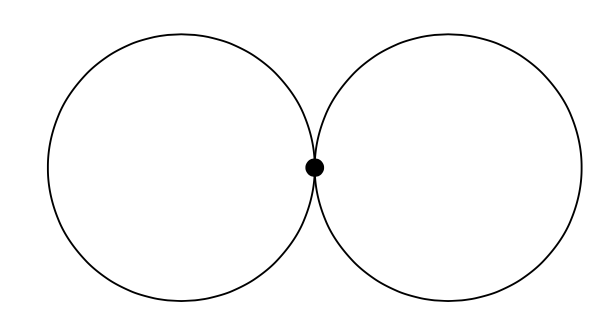
\includegraphics[scale =0.5]{fotos_topo_2/otrasfotos/uniopuntual2circumferencies.png}
\end{equation}
Ara hem d'agafar els oberts $U$ i $V$ i el punt $x_0$ serà el punt d'intersecció de les dues circumferències.
\begin{equation}
    \notag
    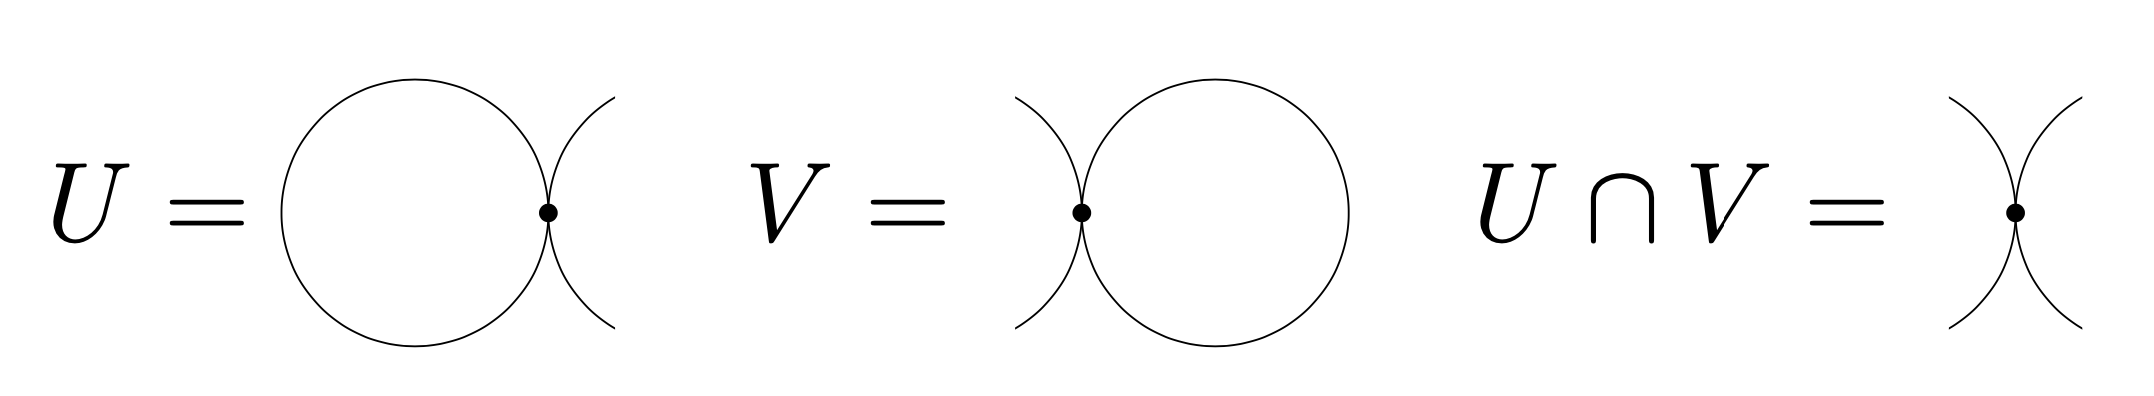
\includegraphics[scale = 0.2]{fotos_topo_2/otrasfotos/UVuniopuntualcirc.png}
\end{equation}
Veiem que, efectivament, $U$ i $V$ són arc-connexos i que $X = U\cap V$. Ara hem de calcular tots els grups fonamentals. Observem que tant $U$ com $V$ són homotòpicament equivalents a $S^1$ i per tant, $\pi(U,x_0)\cong \mathbb{Z} = \langle a\rangle$ i $\pi(V,x_0)\cong \mathbb{Z}= \langle b\rangle$. Finalment, $U\cap V$ és homeomorf a un punt, és a dir, és contràctil. Per tant, $\pi(U\cap V,x_0)\cong\{1\}$. Tenim, doncs, el següent diagrama:
\begin{equation}
    \notag
    \xymatrix{
    \pi(U\cap V,x_0)\cong \{1\} \ar[r]^{\iota_1} \ar[d]^{\iota_2} & \pi(U,x_0)\cong\langle a\rangle \\
    \pi(V,x_0)\cong\langle b\rangle &
    }
\end{equation}
i aleshores, $\pi(X,x_0)$ tindrà com a generadors els generadors de $\pi(U,x_0)$ i de $\pi(V,x_0)$, és a dir, $a$ i $b$; i com a relacions les relacions de $\pi(U,x_0)$, $\pi(V,x_0)$ i les relacions d'amalgament, que són $\iota_1(c) = \iota_2(c)$. Com que $\pi(U,x_0)$ i $\pi(V,x_0)$ no tenen relacions, només ens quedarem amb les relacions d'amalgament. Com que $\pi(U\cap V,x_0)\cong\{1\}$, $\iota_1$ i $\iota_2$ només poden tenir imatges de 1 i com que són morfismes, ha de ser $\iota_1(1) = \iota_2(1) = 1$, ergo, no hi ha relacions d'amalgament tampoc. Aleshores, només ens quedem amb els generadors i el que obtenim és un grup amb dos generadors i cap relació, és a dir, un grup lliure d'ordre 2:
\begin{equation}
    \notag
    \pi(X,x_0)\cong\langle a,b\rangle \cong F_2
\end{equation}
\end{ej}


\begin{ej}
\label{ej:grupfonamentaldeltor} Un altre grup fonamental que podem calcular a través del teorema de Seifert-Van Kampen és el del tor. Comencem representant el tor a partir d'un quadrat amb els seus costats. El punt centre l'anomenarem $x_0$.
\begin{equation}
    \notag
    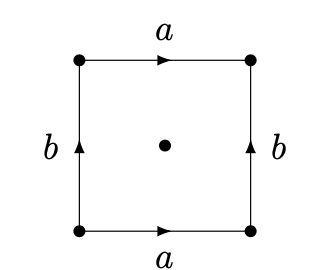
\includegraphics[scale = 0.5]{fotos_topo_2/otrasfotos/exemplegruptor.png}
\end{equation}
Si agafem els oberts següents: $U$ un disc obert que conté el punt $x_0$ i $V = \mathbb{T}^2\setminus\{x_0\}$, aleshores $\mathbb{T}^2 = U\cup V$ i $U\cap V = U\setminus\{x_0\}$, que és un disc obert sense un punt (i per tant és un obert). Ara calculem els seus grups fonamentals. Sigui $p\not=x_0$ un punt de l'interior del disc obert; aleshores $\pi(U,p) = \{1\}$ perquè $U$ és contràctil, per ser homeomorf a $\mathbb{D}^2$. Sigui $q$ el vèrtex de la representació del tor, observem que $V$ es pot retraure al contorn de la representació\footnote{És una mica difícil de veure-ho, però la idea és que ara tenim el quadrat ``buit'' i aleshores identifiquem igualment els costats segons les fletxes, de manera que es generen com dos filferros. Primer identifiquem $a$, aleshores tenim que les dues $b$ formen dues circumferències de filferro unides pel filferro recte resultant d'ajuntar els dos costats $a$. Seguidament, identifiquem les dues circumferències de filferro $b$ que aleshores s'ajunten fent coincidir el punt amb el qual estaven unides a $a$. D'aquesta manera queden dues circumferències de filferro unides, que podem moure per posar-les ``al mateix plà'' i obtenir així $S^1\vee S^1$.}, és a dir que
\begin{equation}
    \notag
    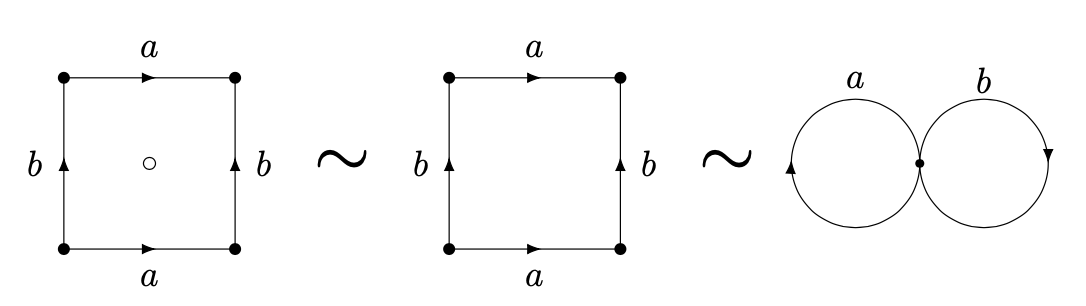
\includegraphics[scale = 0.5]{fotos_topo_2/otrasfotos/exemplegruptor2.png}
\end{equation}
Per tant, recuperant l'exemple anterior, obtenim que $\pi(V,x_0)\cong \langle a,b\rangle$. Finalment, $U\cap V$ és clarament homeomorf a $S^1$ i per tant, $\pi(U\cap V,x_0)\cong \pi(S^1)\cong \mathbb{Z} = \langle c\rangle$. El diagrama d'inclusions queda així:
\begin{equation}
    \notag
    \xymatrix{
    \pi(U\cap V,x_0)\cong\langle c\rangle \ar[r]^{\iota_1}\ar[d]^{\iota_2} & \pi(U,x_0)\cong \{1\} \\
    \pi(V,x_0)\cong\langle a,b\rangle
    }
\end{equation}
aleshores $\iota_1(c) = 1$, $\forall c\in\mathbb{Z}$ ja que ha d'enviar el neutre al neutre i la seva única imatge és el neutre. D'altra banda, $\iota_2$ ens dóna una mica més de problemes. Observem quina és la imatge de $\iota_2(c)$, per a $c\in\mathbb{Z}$. Aquesta inclusió és el camí que recorre, des del vèrtex inferior esquerre, tota la vora del quadrat en sentit antihorari. Això és $\iota_2(c) = aba^{-1}b^{-1}$. Per tant, com que les relacions d'amalgament són $\iota_1(c) = \iota_2(c),\;\forall c\in\pi(U\cap V,x_0)$, obtenim les relacions $aba^{-1}b^{-1} = 1$, és a dir, $ab=ba$. Tenim doncs, 
\begin{equation}
    \notag
    \pi(X,x_0) = \pi(\mathbb{T}^2,x_0)\cong\langle a,b\;:\;ab=ba\rangle = \langle a,b\;:\;aba^{-1}b^{-1}\rangle
\end{equation}
és el grup lliure abelià generat per 2 elements, que és isomorf a $\mathbb{Z}^2$.
Nota. La primera manera d'escriure el grup és la que jo utilitzaria. No obstant, se sol utilitzar la segona manera, ja que així s'indica la paraula que genera el grup. S'omet posar $aba^{-1}b^{-1} = 1$ i es posa directament la paraula només.
\end{ej}















\end{document}